\chapter{Strängars rörelse i vätskor}

Aktinfilament är polymerer som utgör en viktig byggsten i cellens cytoskelett och agerar transportväg för motorprotein. De bidrar därmed till att forma cellens utseende, dynamik och stadga. För att kunna ge en mer detaljerad beskrivning av dessa egenskaper är studien av enstaka aktinfilaments dynamik av stort intresse. 

I det här kapitlet studeras olika dynamiska egenskaper för aktinfilament i en miljö utanför cellen. Studien omfattar både filament som tillåts fluktuera fritt och de som är instängda i en rektangulär kvasi-2D-mikrokanal -- en kanal med försumbart djup. Mikrokanalen är till för att simulera beteendet hos aktinfilament i cytoskelettet där det omges av andra filament och därmed har en begränsad möjlighet till rörelse. Vidare underlättar mikrokanalerna att hålla strängarna i mikroskopets fokalplan.

Det här kapitlet börjar med en översikt över hur mikroskopidatan behandlas för att kunna användas i studien av strängarna. Därefter presenteras och undersöks en WLC-modellen för fria strängrörelser samt en modifikation av modellen som även beskriver inneslutna strängar. I brist på statistiskt underlag är visade det sig vara svårt att avfärda eller bekräfta denna modellen som en förklaring för aktinfilamentens rörelse. De tydligaste skillnaderna är den förhöjda styvheten, persistence length, för instängda strängar vilket inte anses vara i motsägelse med WLC-modellen.

Till sist beskrivs en undersökning av strängarnas egenmoder vars relation mellan vågtal och relaxationstid studeras och presenteras. Dock ska det återigen noteras att mer statistiskt underlag behövs för att tydliga bekräfta detta samband. Egenmoderna för strängarna tas fram på två sätt, där speciellt egenmoder framtagna via diagonalisering av en kovariansmatris sticker ut. Dessa egenmoder visas ha egenskaper likt harmoniska svängningar, vilket utgör den andra studerade utvecklingen av rörelsen i egenmoder, och studien tyder på att en mer teoretiskt koppling mellan modell och kovariansmatrisen kan vara av intresse. 

\section{Undersökt data}
Datan som analyseras för strängrörelse i vätska är den samma som Köster et~al.~\cite{Koster_etal2005,Koster_etal2007,Koster_etal2008} använde. Den består av filmer av aktinfilament som tillåts röra sig i en vätska. Dessa strängar hade en längd på kring 10--30\,\micro{m} och befann sig i olika breda mikrokanaler. 

Två typer av strängar studeras: fria strängar i breda kanaler och inneslutna strängar i en kvasi-2D-mikrokanal. Upplösning på filmerna är 10 bilder per sekund. I båda fallen rörde sig strängarna till största del i två dimensioner då kanalernas djup var litet i förhållande till kanalernas och filamentens bredd.


\subsection{Polynomanpassning för strängarna} \label{sec:polynomanpassning}

\begin{figure}\centering
% GNUPLOT: LaTeX picture with Postscript
\begingroup
  \makeatletter
  \providecommand\color[2][]{%
    \GenericError{(gnuplot) \space\space\space\@spaces}{%
      Package color not loaded in conjunction with
      terminal option `colourtext'%
    }{See the gnuplot documentation for explanation.%
    }{Either use 'blacktext' in gnuplot or load the package
      color.sty in LaTeX.}%
    \renewcommand\color[2][]{}%
  }%
  \providecommand\includegraphics[2][]{%
    \GenericError{(gnuplot) \space\space\space\@spaces}{%
      Package graphicx or graphics not loaded%
    }{See the gnuplot documentation for explanation.%
    }{The gnuplot epslatex terminal needs graphicx.sty or graphics.sty.}%
    \renewcommand\includegraphics[2][]{}%
  }%
  \providecommand\rotatebox[2]{#2}%
  \@ifundefined{ifGPcolor}{%
    \newif\ifGPcolor
    \GPcolortrue
  }{}%
  \@ifundefined{ifGPblacktext}{%
    \newif\ifGPblacktext
    \GPblacktexttrue
  }{}%
  % define a \g@addto@macro without @ in the name:
  \let\gplgaddtomacro\g@addto@macro
  % define empty templates for all commands taking text:
  \gdef\gplbacktext{}%
  \gdef\gplfronttext{}%
  \makeatother
  \ifGPblacktext
    % no textcolor at all
    \def\colorrgb#1{}%
    \def\colorgray#1{}%
  \else
    % gray or color?
    \ifGPcolor
      \def\colorrgb#1{\color[rgb]{#1}}%
      \def\colorgray#1{\color[gray]{#1}}%
      \expandafter\def\csname LTw\endcsname{\color{white}}%
      \expandafter\def\csname LTb\endcsname{\color{black}}%
      \expandafter\def\csname LTa\endcsname{\color{black}}%
      \expandafter\def\csname LT0\endcsname{\color[rgb]{1,0,0}}%
      \expandafter\def\csname LT1\endcsname{\color[rgb]{0,1,0}}%
      \expandafter\def\csname LT2\endcsname{\color[rgb]{0,0,1}}%
      \expandafter\def\csname LT3\endcsname{\color[rgb]{1,0,1}}%
      \expandafter\def\csname LT4\endcsname{\color[rgb]{0,1,1}}%
      \expandafter\def\csname LT5\endcsname{\color[rgb]{1,1,0}}%
      \expandafter\def\csname LT6\endcsname{\color[rgb]{0,0,0}}%
      \expandafter\def\csname LT7\endcsname{\color[rgb]{1,0.3,0}}%
      \expandafter\def\csname LT8\endcsname{\color[rgb]{0.5,0.5,0.5}}%
    \else
      % gray
      \def\colorrgb#1{\color{black}}%
      \def\colorgray#1{\color[gray]{#1}}%
      \expandafter\def\csname LTw\endcsname{\color{white}}%
      \expandafter\def\csname LTb\endcsname{\color{black}}%
      \expandafter\def\csname LTa\endcsname{\color{black}}%
      \expandafter\def\csname LT0\endcsname{\color{black}}%
      \expandafter\def\csname LT1\endcsname{\color{black}}%
      \expandafter\def\csname LT2\endcsname{\color{black}}%
      \expandafter\def\csname LT3\endcsname{\color{black}}%
      \expandafter\def\csname LT4\endcsname{\color{black}}%
      \expandafter\def\csname LT5\endcsname{\color{black}}%
      \expandafter\def\csname LT6\endcsname{\color{black}}%
      \expandafter\def\csname LT7\endcsname{\color{black}}%
      \expandafter\def\csname LT8\endcsname{\color{black}}%
    \fi
  \fi
  \setlength{\unitlength}{0.0500bp}%
  \begin{picture}(6802.00,2834.00)%
    \gplgaddtomacro\gplbacktext{%
    }%
    \gplgaddtomacro\gplfronttext{%
      \csname LTb\endcsname%
      \put(3834,2352){\makebox(0,0)[r]{\strut{}Rådata}}%
      \csname LTb\endcsname%
      \put(3834,2132){\makebox(0,0)[r]{\strut{}Polynomanpassning}}%
      \csname LTb\endcsname%
      \put(3834,1912){\makebox(0,0)[r]{\strut{}Kubisk splineinterpolation}}%
    }%
    \gplbacktext
    \put(0,0){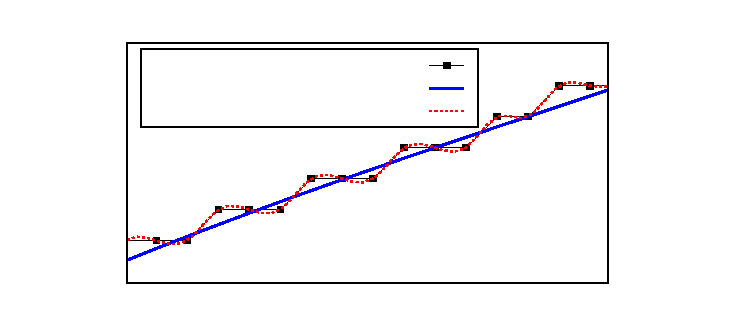
\includegraphics{strang_anpassning}}%
    \gplfronttext
  \end{picture}%
\endgroup

\caption{
Utdrag med pixelpositioner från en av strängarna tillsammans med polynomanpassningen som användes i denna studie samt en spline mellan pixlarna. Utdraget är gjort för en mycket liten del av strängen för att enskilda pixlar ska synas.
Eftersom exempelvis tangent- och normalvektorer till strängarna är intressanta att studera behövs mjuka anpassningar till rådatan så att det går att derivera längs med strängen. 
}
\label{fig:strang_anpassning}
\end{figure}

Mätdatan för strängarna bestod vid varje tidpunkt av en matris med element motsvarande pixlarna på kameran. Datan var förbehandlad och strängen representerades som ett antal 1:or i en annars tom matris. 
För att kunna arbeta effektivt med strängarna behövs dock någon form av anpassning till dessa ''pixlar''. Bland annat behövs mjuka anpassningar för att kunna ta fram tangent- och normalvektorer i en godtycklig punkt längs med strängen. Mjuka anpassningar är även en mer rimlig representation av strängen. I \figref{fig:strang_anpassning} visas ett litet utdrag av en sträng med pixelpositioner och anpassningar. 

För att kunna göra en anpassning behövs först och främst en parameter som kan användas för att anpassas mot. 
Strängens position i varje tidsögonblick parametriserades med en båglängdsparameter $s\in[0,L]$. Alltså svarar $s$ mot hur långt längs med strängen en viss punkt ligger. 
För att i MATLAB bilda båglängdsparametern sorterades först punkterna i en ordnad följd. Efter detta uppskattades hur långt längs med strängen varje pixel låg genom att ackumulera längderna på de förbindande linjerna mellan dem. På så sätt erhölls ett $s$-värde för varje pixel och en anpassning kunde göras av pixlarnas $x$- och $y$-koordinater mot~$s$.

I den här studien valde vi att anpassa positionerna i varje tidpunkt med ett polynom av grad $20$ för $x_t$ och $y_t$ separat enligt
\begin{equation}\label{eq:anpassning}
x_t(s) = \sum_{n=0}^{20} a_n^{(t)} \,s^n,
\end{equation}
där koefficienterna $a_n^{(t)}$ anpassades med hjälp av MATLABs \texttt{polyfit}-funktion till varje pixels position och $s$-värde. På samma sätt kunde även ett polynom för $y$ anpassas. Att det skulle krävas ett 20-gradspolynom för att följa strängen syns inte i \figref{fig:strang_anpassning} på grund av att figuren bara visar en mycket liten del av strängen. Graden behövde dock vara så hög för att de anpassade polynomen skulle kunna följa strängen väl längs med hela strängen. 

Dock får graden inte väljas mycket högre än cirka 20 om man vill undvika andra artefakter från polynomanpassning, som exempelvis en variant av Runges fenomen\cite{Gustafsson_LaNa}. Alltså att polynomet börja svänga kraftigt för att exakt gå igenom alla punkter som det ska anpassas till. Detta är i regel ett problem för interpolationer och inte anpassningar, men om gradtalet väljs ungefär lika stort som antalet punkter som ska anpassas så tenderar anpassningen att bli mer lik en interpolation.


\subsection{Mäta avstånd från jämviktsläge}

\begin{figure}
\centering
\resizebox{0.8\textwidth}{!}{
    \input{bilder/strangar/transv_avst.pdf_t}
}
\caption{Schematisk skiss av hur transversella avståndet från medelsträngen mäts. I varje tidpunkt jämförs medelsträngens position, $\mathbf{r}_0(s)$, med den momentana strängens position, $\mathbf{r}(s, t)$, för samma $s$-värde -- $s$ är en parameter som motsvarar en viss sträcka längs med strängen. För att få ett avståndsmått som kan växla tecken undersöks projiceringen av skillnaden i ortsvektor på medelsträngens normalvektor. 
}
\label{fig:transv_avst}
\end{figure}

Strängens translationsrörelse har till stor del försummats genom att i varje tidpunkt placerat strängens masscentrum i origo. Vid visuell inspektion tycker vi att det ser ut som att strängarna fluktuerar kring ett jämviktsläge. En uppskattning av jämviktsläget $\mathbf{r}_0(s)$ tas fram genom att beräkna medelvärdeskurvan som representerar strängrörelsen. 

Från detta jämviktsläge har det transversella avståndet beräknats enligt 
\begin{equation}
A_s(t) = \mathbf{n}_0(s)\cdot\Big(\mathbf{r}(s,t)-\mathbf{r}_0(s)\Big),
\end{equation}
där $\mathbf{n}_0(s)$ är en normerad normalvektor till strängens jämviktsläge samt $\mathbf{r}(s,t)$ och $\mathbf{r}_0(s)$ är ortsvektorerna för momentansträngen respektive medelsträngen. Avståndet $A_t(s)$ motsvarar alltså projektionen av $(\mathbf{r}(s,t)-\mathbf{r}_0(s))$ på normalvektorn. Detta 
illustreras i \figref{fig:transv_avst}.



\section{Modeller för strängrörelser}

Aktinfilament, precis som tidigare studerade partiklar, påverkas av diffusionsprocesser inuti celler. Således krävs stokastiska modeller för att beskriva rörelsen. En vanligt använd modell inom polymerfysiken är worm-like chain som beskrivs nedan. Denna modell byggs sedan ut för att fånga fler egenskaper hos strängarna samt för att studera hur införandet av en mikrokanal påverkar strängarna. 



\subsection{Worm-Like Chain (WLC)}\label{WLCmodel}

Worm-like chain \cite{Milstein2013} (WLC) är en modell som ämnar beskriva en semiflexibel polymers fluktuationer. I den här modellen antas att polymeren är helt oelastisk, enbart påverkas av termiskt brus och är styv på små längdskalor. 

Om polymeren fluktuerar fritt %utan att vara instängd i en mikrokanal 
ges en minimalistisk WLC-beskrivning av att filamentets fluktuationer regleras av böjningsenergin. För en polymer med $N$ segment, vardera med riktningsvektor $\Delta\mathbf{r}_i$ och längd $\abs{\Delta\mathbf{r}_{i}}=l$, samt böjstyvhet $\kappa$ ges böjningsenergin av
\begin{equation}
    H = -\kappa\sum_{i=1}^{N-1} (\Delta\mathbf{r}_{i}) \cdot (\Delta\mathbf{r}_{i+1}).
\end{equation}
Maximalt bidrag till energin från två på varandra följande segment fås alltså om dessa är antiparallella. 

Givet identiteten $\mathbf{a}\cdot\mathbf{b}=\big(\mathbf{a^2}+\mathbf{b}^2-(\mathbf{a}-\mathbf{b})^2\big)/2$, kan summan skrivas om som en integral i gränsen då $N\to\infty$, $\kappa\to\infty$, $l \to 0$, men där produkten $\kappa{}l$ är finit. Böjningsenergin fås då som 
\begin{equation}\label{böj}
    \frac{H}{\kbT}=\frac{L_\text{p}}{2}\int_{0}^{L}\!\dd{s}\,(\partial_{s}\mathbf{t}(s))^2,
\end{equation}
där $\mathbf{t}(s)$ är enhetstangentvektorn längs med polymeren, $s$ är en båglängdsparameter, och $L_\text{p}=\frac{\kappa l}{\kbT}$ kallas \emph{persistence length}. Parametern $L_\text{p}$ definierar ett mått på strängens flexibilitet och fås som kvoten mellan polymerens böjstyvhet och den termiska energin hos fluiden. 
Detta är den kontinuerliga WLC-modellen \cite{Fixman_WLC1973}. Modellen ger en bra approximation av en polymer där längden av varje enskild molekyl kan försummas. 



\subsection{Utvidgning av WLC-modellen} \label{WLCkanal}

En mer sofistikerad modell kan konstrueras, så att den tar hänsyn till mikrokanalens egenskaper och dess dynamik. I den här utvidgningen beskrivs interaktionen mellan strängen och kanalens väggar som rent sterisk \cite{Koster_etal2007}, alltså att det finns en mjuk potential. 
Inför därför kraften $F \propto A(s)$, där $A(s)$ svarar mot strängens vinkelräta avstånd från centrum av kanalen. Detta leder till att interaktionen kan approximeras med en parabolisk potential. 

För att kunna beskriva kanalens bredd väljs kraften så att medelvärdet längs med strängen och i tid blir
\begin{equation}\label{jäm1}
\ev{\frac{1}{L}\int_{0}^{L}\dd{s} \, A(s)^{2}}=R^2,
\end{equation}
där $R$ är mikrokanalens halva bredd -- som en ''radie''. Den potentiella energin med avseende på de vinkelräta fluktuationerna blir nu~\cite{Harnau&Reineker1999}
\begin{equation}
    \frac{H_{p}}{\kbT}=\frac{\nu}{2L_\text{p}^3}\int_{0}^{L} \!\dd{s} \, A(s)^2,
\end{equation}
där $\nu$ är en dimensionslös Lagrangemultiplikator.

Låt nu $\mathbf{r}(s)$ beteckna strängens position längs båglängdsparametern $s$. Tidigare, i avsnitt~\ref{WLCmodel}, antogs det att polymeren var lokalt inelastiska, vilket är ekvivalent med att $\abs{\partial_{s}\mathbf{r}(s)}^2\equiv1$. Detta försvårar dock beräkningen av strängens jämviktstillstånd. Betrakta därför följande uttryck
\begin{equation}\label{jäm2}
\ev{\int_{0}^{L}\dd s[\partial_{s}\mathbf{r}(s)]^2}=L,
\end{equation}
som istället säger att strängen är globalt inelastisk. Segment av strängen, $[\pd_s\mathbf{r}(s)]^2\!\dd{s}$, kan då variera sin längd var för sig, men väntevärdet av den totala längden är ändå konstant. Fysikaliskt kan detta associeras med en fjäderkraft längs strängen. Inför därför den potentiella energin med avseende på denna kraft enligt \cite{Harnau&Reineker1999} som
\begin{equation}
\frac{H_{f}}{\kbT}=\frac{\mu}{L_\text{p}}\int_{0}^{L}\dd s\,[\partial_{s}\mathbf{r}(s)]^{2},
\end{equation}
där $\mu$ är ytterligare en dimensionslös Lagrangemultiplikator.

Strängens totala potentiella energi fås genom att summera de individuella bidragen från mikrokanalens potential samt strängens böjstyvhet och fjäderkraft. Eftersom tangentvektorn till strängen definieras som $\mathbf{t}(s)=\partial_{s}\mathbf{r}(s)$ fås att
\begin{equation}
\label{Htot}
    \frac{H_\text{tot}}{\kbT}=\int_{0}^{L}\!\dd{s}\,\left[\frac{L_\text{p}}{2}\left(\partial_{s}^{2}\mathbf{r}(s)\right)^2 + \frac{\nu}{2L_\text{p}^3} A(s)^{2}+\frac{\mu}{L_\text{p}}\left(\partial_{s}\mathbf{r}(s)\right)^{2}\right],
\end{equation}
där den första termen i integranden svarar mot energin enligt den tidigare modellen \eqref{böj}, nu betraktad med avseende på strängens position $\mathbf{r}(s)$.

I bilaga~\ref{A5} studeras med variationskalkyl hur den potentiella energin påverkas av en liten störning $\delta A$. Därur erhålls en modell av den återställande kraften på strängen orsakad av termiska fluktuationer. Dessa termiska fluktuationer kan betraktas som en stokastisk brusterm. Alltså kan man, likt i avsnitt~\ref{sec:brown}, studera strängrörelsen med en Langevinekvation \cite{Bullerjahn2011}. Denna ges av 
\begin{equation}\label{mikrokanel}
\zeta\partial_{t}A=-\frac{\delta H_\text{tot}}{\delta A}+\sigma\partial_{t}W,
\end{equation}
där $\zeta$ är en friktionskoefficient per längdenhet av strängen och $\pd_tW(t,s)$ är vitt brus som i \eqref{eq:white_noise}. 
Här ger $-\frac{\delta H_\text{tot}}{\delta A}$ en återställande kraft orsakad av fluktuationer som verkar på längdelementet $\dd{s}$, vilket enligt bilaga \ref{A5} ges av \
\begin{equation}
F=-\frac{\delta H_\text{tot}}{\delta A} = \kbT\left[-L_\text{p}\pd_s^4A-\frac{\nu}{L_\text{p}^3}A+\frac{2\mu}{L_\text{p}}\pd_s^2A \right]\dd{s} .
\end{equation}

%%%%%%%%%%%%%%%%%%%%%%%%%%%%%%%%%%%%%%%%%%%%%%%%%%%%%%%%%%%%%%%%%%%%%%%%%%%
\begin{comment}
\subsubsection{Fenomenologisk modell för en brownsk sträng}\todo[color=red]{Namn? Måns hade kallat den Brownian string.}
\todo[color=red]{Tycker intro ser bra ut. Lite osäker på om man ska använda 'kraftterm', kanske bättre att bara skriva typ: en term med styrka ... Tänker mest på att det blir så konstiga enheter på konstanterna om man ska kalla det för kraftterm.}
Med inspiration från modellen tidigare härledd utifrån strängens potentiella energi kan en alternativ fenomenologisk modell konstrueras. Likt tidigare approximeras mikrokanalens begränsande egenskaper med en parabolisk potential, inför därför en kraftterm proportionell mot strängens vinkelräta avstånd från centrum av kanalen. Dess styrka sätts att vara proportionell mot parametern $\gamma$. Strängen antas likt \eqref{böj} även lagra potentiell energi då denna böjs och därmed ha jämviktsläge likt en stavformation. Intruducera därför en kraftterm kopplad till strängens krökning vars styrka styrs av parametern $\alpha$. I fallet då strängens intrinsiska tröghet, svarandes mot högre ordningens tidsderivata, försummas fås
\todo{okej intro?}
\todo[color=olive]{i detta kapitel skall $\xi$ skrivas om till $\alpha$. :)}
\begin{equation}
\label{mans}
    \partial_{t}A(t,s)=-\zeta A(t,s)+\alpha \partial_{s}^{2}A(t,s)+\sigma \partial_{t}W(t,s).
\end{equation}
Fluktuationerna approximeras här igen med termen $\sigma\partial_{t}W(t,s)$, ett stokastiskt vitt brus. De modellerande konstanterna antas alla vara positiva.

% För att lösa denna stokasktiska PDE introduceras följande fouriertransform 
% \begin{equation}
%     \hat{A}(t,k)=\int_{-\infty}^{\infty}\!\dd{s}\, A(t,s)\ee^{-\ii sk}
% \end{equation}

Genom fouriertransformation av \eqref{mans} fås en ordinär stokastisk differentialekvation av första ordningen
\begin{equation}
        \partial_{t}\hat{A}(t,k)=-\left(\gamma+\xi k^2\right)\hat{A}(t,k)+\sigma \partial_{t}\hat{W}(t,k).
\end{equation}
I fallet då $\gamma+\xi k^2=\zeta$ ses det att denna ekvation är ekvivalent med \eqref{eq:Brownian_SDE} vars lösning är känd. Vidare kan kovariansen formuleras likt \eqref{Brownian_korr}. Då fås att
\begin{equation}\label{jobbig}
\begin{aligned}
    \ev{\hat{A}(t,k)\hat{A}(t',k')} =& \ev{\hat{A}(0,k)\hat{A}(0,k')} \ee^{-(\gamma+\xi k^2)(t+t')}\\ 
    &+ \sigma^2 \int_{0}^{t}\int_{0}^{t'}\!\dd\tau\dd\tau' \ee^{(\gamma+\xi k^2)(\tau+\tau')} \ev{\partial_{t}\hat{W}(\tau,k)\partial_{t}\hat{W}(\tau',k')}.
\end{aligned}
\end{equation}
Integralen i \eqref{jobbig} beror på vitt brus i fourierrummet $\hat{W}(t,k)$. Denna beräknas genom fouriertransformation av \eqref{eq:white_noise}, vilket ger
\begin{equation}
    \ev{\partial_{t}\hat{W}(t,k)\partial_{t}\hat{W}(t',k')}=\delta(t-t')\delta(k+k').
\end{equation}

Insättning av detta resultat i \eqref{jobbig} samtidigt som ekvationen betraktas i gränsen då $t, t'\rightarrow\infty$ medan $\Delta t=\abs{t-t'}$ hålls finit ger
\begin{equation}
    \ev{\hat{A}(t,k)\hat{A}(t',k')}=\frac{\sigma^2}{2(\gamma+\xi k^2)}\delta(k+k')\ee^{(\gamma+\xi k^2)\abs{t-t'}}.
\end{equation}
Slutligen återfås kovariansen för de rumsliga variablerna $s$ och $s'$ genom invers fouriertransform
\begin{equation}
\label{2korr}
    \ev{A(t,s)A(t',s')}=\frac{\sigma^2}{(2\pi)^2\sqrt{\gamma\xi}}\int_{-\infty}^{\infty}\!\dd{p} \frac{\exp[-(1+p^2)\gamma \abs{t-t'}+\ii p\sqrt{\frac{\gamma}{\xi}}(s-s')]}{1+p^2},
\end{equation}
där variabeln $p$ är en hjälpvariabel $\nicefrac{\dd{p}}{\dd{k}}=\sqrt{\frac{\xi}{\gamma}}$. 

Då kovariansen beror på differensen mellan variablerna $\Delta t=t-t'$ samt $\Delta s=s-s'$ är denna translationsinvariant. Det kan visas då för en godtycklig förflyttning i tiden $\delta{t}$ fås att $\ev{A(t,s)A(t',s')}=\ev{A(t+\delta t,s)A(t'+\delta t,s')}$. Därmed kan tvåpunktkorrelationen för \eqref{mans} definieras som
\begin{equation}
    \kappa (\Delta t,\Delta s)=\frac{\ev{A(\Delta t,\Delta s)A(0,0)}}{\ev{A(0,0)^2}}.
\end{equation}
\end{comment}
%%%%%%%%%%%%%%%%%%%%%%%%%%%%%%%%%%%%%%%%%%%%%%%%%%%%%%%%%%%%%%%%%%%%%%%%%%%



\section{Tangentkorrelation}

Korrelationen mellan två tangentvektorer beräknade från den minimalistiska WLC-modellen fås genom att studera \eqref{böj} medelvärdsbildad över tid. Man får då \cite{Landau1958}
\begin{equation} \label{eq:tangentkorr_exp}
\ev{\mathbf{t}(s)\mathbf{t}(s+\Delta s)}=\ee^{-\frac{\abs{\Delta s}}{2L_\text{p}}},
\end{equation}
där $L_\text{p}$ är \emph{persistence length} som ger ett mått på hur snabbt tangentkorrelationen avtar längs polymeren. 

För att öka noggrannheten kan även ett rumsligt medelvärde tas över tangentkorrelationen; låt detta betecknas med ett heldraget streck. Tangentkorrelationen beror då inte längre av var på strängen korrelationen betraktas utan bara på avståndet mellan tangentvektorerna, $\Delta s$, och definieras som
\begin{equation}
\label{tangkorr}
    \ev{\cos(\theta(\Delta s))}\equiv\overline{\ev{\mathbf{t}(s)\mathbf{t}(s+\Delta s)}}.
\end{equation}

Den minimalistiska WLC-modellen förutspår alltså tangentkorrelationens utseende utifrån antagandet att strängen tillåts fluktuera fritt. Genom att beräkna tangentkorrelationen för både fria och instängda strängar kan mikrokanalens inverkan på strängen studeras. Vidare ger tangentkorrelationen ett mått på hur väl strängen motverkar böjning, i fallet då $\nicefrac{L_\text{p}}{L}\gg1$ sägs polymeren vara styv. 



\subsection{Resultat -- mikrokanalen ökar tangentkorrelationen}

Tangentkorrelationen beräknas enligt \eqref{eq:tangentkorr_exp} och plottas i \figref{fig:tangentkorr} för en fri och en instängd sträng. För den fria strängen beräknas persistence length till cirka $L_\text{p}=\unit[50]{\micro{m}}$. Eftersom strängens längd är ungefär \unit[35]{\micro{m}}, är persistence length längre än strängens längd. Därmed kan filamentet anses vara styvt.

%Den fria strängen är alltså styv; tangentvektorn vid en punkt ger statistiskt sett information om tangentvektorn i en godtycklig punkt längs strängen. %Tangentkorrelationen för den instängda strängen följer inte ett exponentialsamband. Alltså kan inte en persistence length uppskattas från \eqref{tangkorr}. Däremot ses en stor tangentkorrelationen utmed hela strängen. Således kan även den instängda strängen vara styv.

Eftersom aktinfilamenten i de olika proverna är snarlika, där den enda signifikanta skillnad är deras längd, reflekterar skillnaden i korrelationsfunktionen mikrokanalens påverkan på strängen. %Den instängda strängen visar en bestående korrelation för större längder än den vad fria strängen gör.
%upplevs ha mycket större persistent length än vad som väntas av ett aktinfilament. %Då persistence length ger ett mått på strängens böjstyvhet och en sträng i en smal mikrokanal begränsas till att fluktuera längs kanalens mitten förklarar det varför tangentkorrelationen är bestående. 

Enligt \eqref{eq:tangentkorr_exp} fås att en sträng ska gå mot att bli okorrelerad för stora avstånd. \figref{fig:tangentkorr} visar dock att tangentkorrelationen för en sträng instängd i en mikrokanal inte avtar exponentiellt utan är bestående; den går snabbt mot ett lokalt minimum och sedan asymptotiskt mot ett konstant värde. %Strängen korrelerar alltså bra för avstånd mycket längre än persistence length för aktinfilament. 
%Strängen är alltså styv; tangentvektorn vid en punkt ger statistiskt sett information om tangentvektorn i en godtycklig punkt längs strängen. 
Detta kan tänkas förklaras med att en sträng i en mikrokanal kolliderar med dess väggar, byter riktning och fortsätter korrelera med punkter långt bort på strängen. 

\begin{figure}
    \centering
    % GNUPLOT: LaTeX picture with Postscript
\begingroup
  \makeatletter
  \providecommand\color[2][]{%
    \GenericError{(gnuplot) \space\space\space\@spaces}{%
      Package color not loaded in conjunction with
      terminal option `colourtext'%
    }{See the gnuplot documentation for explanation.%
    }{Either use 'blacktext' in gnuplot or load the package
      color.sty in LaTeX.}%
    \renewcommand\color[2][]{}%
  }%
  \providecommand\includegraphics[2][]{%
    \GenericError{(gnuplot) \space\space\space\@spaces}{%
      Package graphicx or graphics not loaded%
    }{See the gnuplot documentation for explanation.%
    }{The gnuplot epslatex terminal needs graphicx.sty or graphics.sty.}%
    \renewcommand\includegraphics[2][]{}%
  }%
  \providecommand\rotatebox[2]{#2}%
  \@ifundefined{ifGPcolor}{%
    \newif\ifGPcolor
    \GPcolortrue
  }{}%
  \@ifundefined{ifGPblacktext}{%
    \newif\ifGPblacktext
    \GPblacktexttrue
  }{}%
  % define a \g@addto@macro without @ in the name:
  \let\gplgaddtomacro\g@addto@macro
  % define empty templates for all commands taking text:
  \gdef\gplbacktext{}%
  \gdef\gplfronttext{}%
  \makeatother
  \ifGPblacktext
    % no textcolor at all
    \def\colorrgb#1{}%
    \def\colorgray#1{}%
  \else
    % gray or color?
    \ifGPcolor
      \def\colorrgb#1{\color[rgb]{#1}}%
      \def\colorgray#1{\color[gray]{#1}}%
      \expandafter\def\csname LTw\endcsname{\color{white}}%
      \expandafter\def\csname LTb\endcsname{\color{black}}%
      \expandafter\def\csname LTa\endcsname{\color{black}}%
      \expandafter\def\csname LT0\endcsname{\color[rgb]{1,0,0}}%
      \expandafter\def\csname LT1\endcsname{\color[rgb]{0,1,0}}%
      \expandafter\def\csname LT2\endcsname{\color[rgb]{0,0,1}}%
      \expandafter\def\csname LT3\endcsname{\color[rgb]{1,0,1}}%
      \expandafter\def\csname LT4\endcsname{\color[rgb]{0,1,1}}%
      \expandafter\def\csname LT5\endcsname{\color[rgb]{1,1,0}}%
      \expandafter\def\csname LT6\endcsname{\color[rgb]{0,0,0}}%
      \expandafter\def\csname LT7\endcsname{\color[rgb]{1,0.3,0}}%
      \expandafter\def\csname LT8\endcsname{\color[rgb]{0.5,0.5,0.5}}%
    \else
      % gray
      \def\colorrgb#1{\color{black}}%
      \def\colorgray#1{\color[gray]{#1}}%
      \expandafter\def\csname LTw\endcsname{\color{white}}%
      \expandafter\def\csname LTb\endcsname{\color{black}}%
      \expandafter\def\csname LTa\endcsname{\color{black}}%
      \expandafter\def\csname LT0\endcsname{\color{black}}%
      \expandafter\def\csname LT1\endcsname{\color{black}}%
      \expandafter\def\csname LT2\endcsname{\color{black}}%
      \expandafter\def\csname LT3\endcsname{\color{black}}%
      \expandafter\def\csname LT4\endcsname{\color{black}}%
      \expandafter\def\csname LT5\endcsname{\color{black}}%
      \expandafter\def\csname LT6\endcsname{\color{black}}%
      \expandafter\def\csname LT7\endcsname{\color{black}}%
      \expandafter\def\csname LT8\endcsname{\color{black}}%
    \fi
  \fi
    \setlength{\unitlength}{0.0500bp}%
    \ifx\gptboxheight\undefined%
      \newlength{\gptboxheight}%
      \newlength{\gptboxwidth}%
      \newsavebox{\gptboxtext}%
    \fi%
    \setlength{\fboxrule}{0.5pt}%
    \setlength{\fboxsep}{1pt}%
\begin{picture}(6802.00,3968.00)%
    \gplgaddtomacro\gplbacktext{%
      \csname LTb\endcsname%
      \put(740,640){\makebox(0,0)[r]{\strut{}$0,7$}}%
      \csname LTb\endcsname%
      \put(740,1302){\makebox(0,0)[r]{\strut{}$0,8$}}%
      \csname LTb\endcsname%
      \put(740,1965){\makebox(0,0)[r]{\strut{}$0,9$}}%
      \csname LTb\endcsname%
      \put(740,2627){\makebox(0,0)[r]{\strut{}$1$}}%
      \csname LTb\endcsname%
      \put(860,440){\makebox(0,0){\strut{}$0$}}%
      \csname LTb\endcsname%
      \put(1604,440){\makebox(0,0){\strut{}$2$}}%
      \csname LTb\endcsname%
      \put(2348,440){\makebox(0,0){\strut{}$4$}}%
      \csname LTb\endcsname%
      \put(3092,440){\makebox(0,0){\strut{}$6$}}%
      \csname LTb\endcsname%
      \put(3837,440){\makebox(0,0){\strut{}$8$}}%
      \csname LTb\endcsname%
      \put(4581,440){\makebox(0,0){\strut{}$10$}}%
      \csname LTb\endcsname%
      \put(5325,440){\makebox(0,0){\strut{}$12$}}%
      \csname LTb\endcsname%
      \put(6069,440){\makebox(0,0){\strut{}$14$}}%
    }%
    \gplgaddtomacro\gplfronttext{%
      \csname LTb\endcsname%
      \put(160,1633){\rotatebox{-270}{\makebox(0,0){\strut{}$\ev{\cos{\left(\theta(\Delta s)\right)}}$}}}%
      \put(3650,140){\makebox(0,0){\strut{}$\Delta s$ /[$\micro$m]}}%
      \csname LTb\endcsname%
      \put(5359,3685){\makebox(0,0)[r]{\strut{}95\,\% konfidensintervall}}%
      \csname LTb\endcsname%
      \put(5359,3465){\makebox(0,0)[r]{\strut{}Instängd sträng nr. 1}}%
      \csname LTb\endcsname%
      \put(5359,3245){\makebox(0,0)[r]{\strut{}Fri sträng nr. 1}}%
      \csname LTb\endcsname%
      \put(5359,3025){\makebox(0,0)[r]{\strut{}Exponentialsamband med $L_{\text{p}}=48,6\micro$m}}%
    }%
    \gplbacktext
    \put(0,0){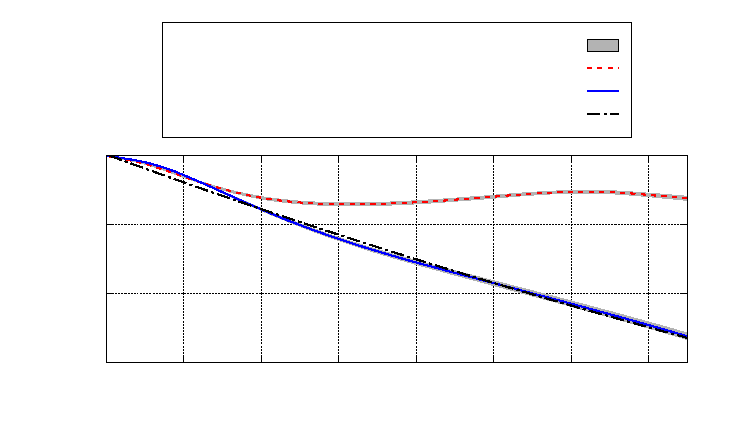
\includegraphics{tangentkorr}}%
    \gplfronttext
  \end{picture}%
\endgroup

    \caption{Tangentkorrelation för en fri sträng och för en instängd sträng med en längd på $\unit[35]{\micro m}$ respektive $\unit[22]{\micro m}$ visas. För den fria strängen anpassas ett exponentialsamband med en persistence length på omkring $L_\text{p} = \unit[50]{\micro m}$. För den instängda strängen avtar korrelationen för att sedan plana ut mot en beständig korrelation längs strängen, därmed plottas ingen exponentialanpassning till denna. Ifall en sådan görs för att beräkna dess styvhet erhålls en persistent length omkring $\unit[300]{\micro m}$. Notera att det finns mindre statistik för den instängda strängen på grund av skillnaden i strängarnas längd.}
    \label{fig:tangentkorr}
\end{figure}

%%%%%%%%%%%%%%%%%%%%%%%%%%%%%%%%%%%%%%%%%%%%%%%%%%%%%%%%%%%%%%%%%%%%%%%%%%%
\begin{comment}
\subsection{Resultat -- (tvåpunktskorrelation)}

Fysikaliska tolkningen av en tvåpunktskorrelationsfunktion är att ge mått på hur snabbt avvikelser från strängens jämviktsläge skingras med tid samt avstånd på strängen. Korrelationen beräknas numeriskt från strängdatan, vilket betraktats i ett godtyckligt antal ekvidistanta diskreta punkter längs strängen, $\Delta s$ är avståndet mellan två efterföljande punkter. Tvåpunktskorrelationen beräknas för data som en normerad kovariansmatris enligt \todo[color=olive]{referera till eq från stoc. kap}. Temporala korrelationen fås genom att studera strängens utveckling i bildspelet, där $\Delta t$ svarar mot tidsintervallet mellan två följande bilder. Kovariansmatrisen härleddes även teoretiskt för strängar begränsade av mikrokanaler \eqref{2korr}. Den teoretiska korrelationen  beräknas för samma temporala samt rumsliga förskjutningar $\Delta s, \Delta t$ som i strängdatan fås den att helt bestämmas av parametrarna $\gamma,\xi,\sigma$. Genom att matcha dessa olika kovariansmatriser erhålls ett mycket överbestämt ekvationssystem ur vilket dessa parametrar kan bestämmas.
\todo{fixa 3D-plots på dessa och förklara deras utseende} \\ \\
Tvåpunktskorrelationen kan även betraktas i två specialfall; då $\Delta t=0$, vilket likt den minimalisktiska WLC modellen svarar mot korrelation längs strängen, samt då $\Delta s=0$, vilket ger temporal korrelation. För båda fallen kan \eqref{2korr} lösas analytiskt, korrelationen längs strängen ges av
\begin{equation}\label{eq:tangentkorr}
\ev{A(s)A(s')}=\exp(-\sqrt{\frac{\gamma}{\xi}}\abs{\Delta s}),
\end{equation}
vilket är samma som tangentkorrelationen \eqref{tangkorr} för minimalistiska WLC-modellen. Motsvarigheten till $L_{\text{p}}$ för en sträng i en mikrokanal som $L_\text{p}=\sqrt{\frac{\xi}{\gamma}}$.
Temporala korrelationen ges av
\begin{equation}
    \ev{A(t)A(t')}=\mathrm{erfc}(\sqrt{\gamma\abs{\Delta t}}),
\end{equation}
där $\mathrm{erfc}(.)$ är \emph{complementary error function} definierad som $\mathrm{erfc}(x)=\frac{2}{\sqrt{\pi}}\int_{x}^{\infty}\ee^{-y^2}\dd y$.

I figur \todo[color=olive]{figur på 2-korr för confined strängar}.. ses ytor svarandes mot tvåpunktskorrelationerna, där den teoretiska modellen anpassats med avseende på parametrarna $\gamma,\xi,\sigma$ för att matcha numeriska korrelationen. 
\end{comment}
%%%%%%%%%%%%%%%%%%%%%%%%%%%%%%%%%%%%%%%%%%%%%%%%%%%%%%%%%%%%%%%%%%%%%%%%%%%




\section{Egenmoder}
Ett vanligt sätt att studera svängningar är att dela upp dem i egenmoder. Genom en linjärkombination av dessa egenmoder kan sedan en godtycklig svängning representeras. 

Anledningen att det är intressant att studera egenmoder är att de är oberoende av varandra. Exempelvis kan en gitarrsträngs svängningar delas upp i sådana oberoende moder. Och eventuellt kan även aktinfilamentens svängningar representeras med hjälp av liknande egenmoder. 

I det här avsnittet studeras därför två sätt att utveckla strängrörelsen i möjliga egenmoder: genom cosinusutveckling och med egenvektorerna till filamentens kovariansmatris, där kovariansmatrisen är konstruerad med strängens transversella avståndskomponenter. 


\subsection{Strängrörelse genom cosinusutveckling} \label{sec:costransform}
Börja med att betrakta \eqref{mikrokanel} som beskriver strängens svängningar. Det kan då tänkas att dess lösningar kan skrivas som en linjärkombination av dess egenfunktioner. Alltså att positionsvektorn kan utvecklas i en bas av egenmoder
\begin{equation}
\label{basutv}
    A(t,s)=\sum_{n=1}^{\infty}a_{n}(t)\psi_{n}(s),
\end{equation}
där $a_{n}(t)$ är egenvärdet till respektive egenmod $\psi_{n}(s)$. 

Värdet på $a_{n}(t)$ svarar mot egenmodens amplitud vilket ansätts vara tidsberoende. Insättning i \eqref{mikrokanel} ger följande differentialekvation 
\begin{equation}\label{egenvard}
\zeta\sum_{n=1}^{\infty}\partial_{t}a_{n}(t)\psi_{n}(s)
= \sigma\partial_{t}W(t,s) +
\kbT\sum_{n=1}^{\infty}
a_{n}(t) \left[
-L_{\text{p}}\partial_{s}^{4}
-\frac{\nu}{L_{\text{p}}^{3}}
+\frac{2\mu}{L_{\text{p}}}\partial_{s}^{2}
\right]\psi_{n}(s).
\end{equation}
Summanden i högerledet svarar mot en differentialoperator verkande på moderna. Ansätt nu $\psi_{n}(s)$ att vara egenvektorer till operatorn, alltså att
\begin{equation}
    \kbT\left[-L_{\text{p}}\partial_{s}^{4}-\frac{\nu}{L_{\text{p}}^{3}}
+\frac{2\mu}{L_{\text{p}}}\partial_{s}^{2}\right]\psi_{n}(s)=-\lambda_{n}\psi_{n}(s),
\end{equation}
där $\lambda_{n}$ är egenvärden till operatorn vilka antas vara tidsoberoende.

Lösningarna till denna egenvärdesekvation ges av sinus- och cosinusfunktioner. Dock eftersträvas enbart lösningar som samtidigt spänner upp en möjlig bas till strängarnas svängningar. Moderna fås enligt \cite{Harnau&Reineker1999} som $\psi_{n}(s)=\cos\left({\frac{n\pi}{L}s}\right)$. Insättning av detta i \eqref{egenvard} reducerar ekvationen till
\begin{equation}
    \sum_{n=1}^{\infty}\left[
    \zeta\partial_{t}a_{n}(t)+\lambda_{n} a_{n}(t)
    \right]\psi_{n}(s)=\sigma\partial_{t}W(t,s).
\end{equation}
Multiplicera båda sidor ovan med $a_n(0)$ för att få en korrelation. Utnyttja sedan att $\ev{\partial_{t}W(t,s)}=0$, vilket ger
\begin{equation}
    \sum_{n=1}^{\infty}\ev{\zeta\partial_{t}a_{n}(t)a_n(0)+\lambda_{n}a_{n}(t)a_n(0)}\psi_{n}(s)=0.
\end{equation}
Eftersom $\psi_{n}(s)$ spänner upp en bas måste $\ev{\zeta\partial_{t}a_{n}(t)a_{n}(0)+\lambda a_{n}(t)a_{n}(0)}=0$. Ur lösningen erhålls korrelationsfunktionerna för modernas amplituder
\begin{equation}
\label{modkorr2}
    \ev{a_{n}(t)a_{n}(0)}=\ee^{-\frac{\lambda_{n}}{\zeta}t}.
\end{equation}
Det fås att korrelationen för svängningsmoderna avtar exponentiellt med en karakteristisk tid $\nicefrac{\zeta}{\lambda_{n}}$. 

För att förenkla denna ekvationen omdefinieras egenvärdena som $\tau_n=\nicefrac{\zeta}{\lambda_n}$, där $\tau_{n}$ är modernas \emph{relaxationstid}. Korrelationen \eqref{modkorr2} fås nu som
\begin{equation}\label{modkorr}
\ev{a_{n}(t)a_{n}(0)}=\ee^{-\frac{t}{\tau_{n}}}.
\end{equation}
Genom att lösa ekvation \eqref{egenvard} för egenmoderna erhålls en ekvation ur vilket tiderna $\tau_{n}$ kan beräknas explicit
\begin{equation}\label{relaxconf}
    \frac{\zeta}{\tau_{n}\kbT}=L_{\text{p}}\left(\frac{n\pi}{L}\right)^{4}+\frac{2\mu}{L_{\text{p}}}\left(\frac{n\pi}{L}\right)^{2}+\frac{\nu}{L_{\text{p}}^3}.
\end{equation}
Relaxationstiden avtar alltså med ordningen på moden. Eftersom den harmoniska potentialen med styrka $\nu$ modellerar den begränsande kanalen så ses enligt denna modell att relaxationstiden för högre ordningens moder påverkas mindre av kanalen än lägre ordningens moder. 

Samma analys kan göras för strängar vars svängningar inte begränsas av mikrokanalen. Då en sådan sträng inte upplever någon harmonisk potential sätts den modellerande konstanten $\nu=0$ i \eqref{relaxconf}. Relaxationstiderna fås då till att enbart bero på ordningen av moden. 
%\begin{equation}\label{relaxnonconf}
 %   \frac{\zeta}{\tau_{n}\kbT}=\frac{2\mu}{L_{\text{p}}}\left(\frac{n\pi}{L}\right)^{2}+L_{\text{p}}\left(\frac{n\pi}{L}\right)^{4}.
%\end{equation}



\subsection{Egenmoder från kovariansmatrisen}

I tidigare avsnitt undersöktes strängens rörelse genom att utveckla denna i en cosinusbas. En annan metod för uppdelning av strängens rörelse i egenmoder beskrivs i avsnitt~\ref{sec:kovmatris} som en diagonalisering av kovariansmatrisen $\mathsf{C}$. I det här fallet konstrueras den av de transversella avstånden $A_s(t)$, där $s$ är en \emph{diskret} båglängdsparameter. Diagonalisering av kovariansmatrisen leder effektivt till ett basbyte från en bas bestående av det transversella avståndet i varje punkt $s$ längs strängen, till en bas bestående av egenmoderna för strängen. 

Egenvärdena till kovariansmatrisen ger ett mått på hur mycket av strängens rörelse som byggs upp av motsvarande egenmod. Framtida användning av storleken på moden avser därför storleken på egenvärdet. I avsnitt~\ref{sec:kovmatris} påpekas även att den tidsmedelvärdesbildade variansen av varje mod svarar precis mot egenvärdena till kovariansmatrisen. Genom att projicera strängens rörelse på ett fåtal av de egenmoder med störst egenvärde förenklas analysen\cite{Shlens_PCA2014}; karakteristiska egenskaper för varje egenmod kan då undersökas separat. 

\subsubsection{Diagonalisering av kovariansmatrisen}
Med diskreta steg längs strängen och i tiden kan varje punkts $A$-värde beskrivas med en uppsättning vektorer
\begin{equation}
\mathbf{A}(t) 
%= \begin{bmatrix}
%A_1(t) &\cdots &A_s(t) & \cdots & A_n(t)
%\end{bmatrix}^\mathsf{T}.
= \Big[
A_1(t) \ldots A_s(t) \ldots A_n(t)
\Big]^\mathsf{T}.
\end{equation}
Alltså att varje $t$-värde ger en ny vektor, och att $A_s(t)$ är det $s$:te elementet i $\mathbf{A(t)}$. 
Kovariansmatrisen beräknas enligt \eqref{eq:kovmatris}:
\begin{equation} 
\label{eq:C}
    \mathsf{C}_{s s'} = \COV{A_s(t)}{A_{s'}(t)}_t.
\end{equation}
För att kunna diagonalisera en matris måste den vara inverterbar~\cite{Gustafsson_LaNa}. Med andra ord så får $\mathsf{C}$ inte ha något egenvärde som är $0$. 

Det är inte självklart att $\mathsf{C}$ bara har nollskilda egenvärden. För att illustrera detta kan man börja med att betrakta en $2\times 2$-kovariansmatris. Om det ena egenvärdet till den är $0$, så betyder det att variansen~\cite{Shlens_PCA2014} i den riktningen är $0$. Genom att betrakta $A_1(t)$ och $A_2(t)$ som punkter i en plan, ger tolkingen att variansen i en viss riktning är $0$ att punkterna befinner sig på en linje\footnotemark{}. De två punkterna skulle då vara \emph{perfekt} korrelerade, vilket är orimligt i en verklig sträng. Det här argumentet har gjorts för enbart två punkter på strängen, men illustrerar varför $\mathsf{C}$ är diagonaliserbar. Det går att utvidga argumentet till fler punkter, men det blir då inte lika tydligt varför det är praktiskt orimligt med ett egenvärde som är $0$. 
\footnotetext{Jämför detta med asfärisiteten i avsnitt~\ref{sec:isotropi}. Om ena egenvärdet hade blivit $0$, så skulle afärisiteten i \eqref{eq:asph._2D} blivit 1, vilket svarar mot en linje i planet.  }

Eftersom $\mathsf{C}$ är diagonaliserbar kommer dess normerade egenvektorer, $\mathbf{B}_i$, att utgöra en ON-bas. Vidare är tolkningen av en diagonalisering av $\mathsf{C}$ att man byter till basen som spänns upp av $\mathbf{B}_i$. I och med det här basbytet erhåller man de nya egenmodernas värde i varje tidpunkt, $b_i(t)$, som projektionerna av $\mathbf{A}(t)$ på $\mathbf{B}_i$. Man får alltså
\begin{equation} \label{eq:egenmod_b}
b_i(t) = \mathbf{A}(t)\cdot\mathbf{B}_i =\sum_{s=1}^n A_s(t)\,B_i^{(s)},
\end{equation}
där $B_i^{(s)}$ är det $s$:te elementet i $\mathbf{B}_i$.

%%%%%%%%%%%%%%%%%%%%%%%%%%%%%%%%%%%%%%%%%%%%%%%%%%%%%%%%%%%%%%
\begin{comment} 
Kovariansmatrisen bildas sedan av $A_s(t)$ enligt \eqref{eq:kovmatris}. Detta ger
\begin{equation}
\label{eq:C}
    \mathsf{C}_{s s'} = \COV{A_s(t)}{A_{s'}(t)}_t.
\end{equation}
Egenvektorerna, även kallade egenmoderna, till $\mathsf{C}$ betecknas $\mathbf{B}_i$ och strängrörelsen kan representeras som
\begin{equation}
    A_s(t) = \sum_i^n \alpha_{si}(t)\mathbf{B_i}.
\end{equation}
%Med $\hat{\mathbf{A}}_s$ som en enhetsvektor för komponent $s$ blir 
Här ges
\begin{equation}
    \alpha_{si}(t) = A_s(t)\mathbf{B}_i\cdot\hat{\mathbf{A}}_s,
\end{equation}
där $\hat{\mathbf{A}}_s$ är enhetsvektorn för komponent $s$. 

Projektionen av strängrörelsen på varje egenmod som funktion av tiden beskrivs av
\begin{equation}
    b_i(t) = \sum_s^n \alpha_{si}(t).
\end{equation}
Alltså är $b_i(t)$ ett mått på hur mycket av strängen som vid tiden $t$ består av egenmod $\mathbf{B_i}$, vilket kan liknas med expansionskofficent vid utveckling av en funktion i fourierserie.
\end{comment} 
%%%%%%%%%%%%%%%%%%%%%%%%%%%%%%%%%%%%%%%%%%%%%%%%%%%%%%%%%%%%%%

\subsubsection{Tolkning av den diagonaliserade kovariansmatrisen}

Vinsten med att ta sig besväret att byta bas till $\mathbf{B}_i$ är att varje egenmods värde $b_i(t)$ är statistiskt okorrelerade. Detta är en följd av att kovariansmatrisen diagonaliseras av basbytet till dess egenvektorer\cite{Gustafsson_LaNa}. Man kan alltså nu undersöka svängningar i strängen som är mer eller mindre statistiskt oberoende. 

Autokorrelationsfunktionen för varje komponent $b_i(t)$ innehåller information om strängrörelsens tidsutveckling. Genom att endast betrakta de komponenter med ''tillräckligt'' stora egenvärden förenklas analysen och relaxationstider för de mest dominanta egenmoderna tas fram från 
\begin{equation}
\label{eq:korrmoder}
    \ev{b_i(t)b_i(t+\Delta t)}_t.
\end{equation}
Antalet egenvärden som är tillräckligt att studera beror på hur väl man vill beskriva rörelsen. Det finns flera modeller för att bestämma hur många egenvärden som behövs, men enligt \cite{Cangelosi2007} så förutspår dessa inte alltid entydiga svar. 

Det går dessutom att hitta en tolkning av egenvektorerna själva. I \eqref{eq:egenmod_b} summeras värden på $A_s$ och $B_i(s)$ över $s$. Men om man låter antalet $s$-värden gå mot oändligheten, så kan summan tolkas som att den övergår i en integral av två funktioner
\begin{equation} \label{eq:egenmoder_fourierkoef}
b_i(t) \to \int_0^L A(s, t)\,B_i(s) \,\dd{s}.
\end{equation}
Jämför detta med hur fourierkoefficienter tas fram i en fourierserie. Den enda skillnaden här är att basfunktionerna har bytts ut från sinus- och cosinusfunktioner till $B_i(t)$. Det finns alltså likheter med den här metoden och att använda cosinustransform för att dela upp strängrörelerna i egenmoder. Detta ger att $B_i(s)$ bör tolkas, på samma sätt som cosinusfunktionerna, som en slags rumslig svängning.


\subsection{Resultat -- det går att mäta en relation mellan vågtal och relaxationstid}
I det här avsnittet har två olika metoder att dela upp strängrörelsen i egenmoder presenterats. De är båda ganska likartade, men bygger på olika utgångspunkter. Erhållna resultat mellan metoderna är snarlika. Detta är en indikation på att egenmoder från kovariansmatrisen har egenskaper som liknar harmoniska svängningar. 


\subsubsection{Cosinustransformen har ett kvalitativt beteende som förutspås av WLC-modellen}

\begin{figure}
    \centerline{
    \subfigure[][]{
    % GNUPLOT: LaTeX picture with Postscript
\begingroup
  \makeatletter
  \providecommand\color[2][]{%
    \GenericError{(gnuplot) \space\space\space\@spaces}{%
      Package color not loaded in conjunction with
      terminal option `colourtext'%
    }{See the gnuplot documentation for explanation.%
    }{Either use 'blacktext' in gnuplot or load the package
      color.sty in LaTeX.}%
    \renewcommand\color[2][]{}%
  }%
  \providecommand\includegraphics[2][]{%
    \GenericError{(gnuplot) \space\space\space\@spaces}{%
      Package graphicx or graphics not loaded%
    }{See the gnuplot documentation for explanation.%
    }{The gnuplot epslatex terminal needs graphicx.sty or graphics.sty.}%
    \renewcommand\includegraphics[2][]{}%
  }%
  \providecommand\rotatebox[2]{#2}%
  \@ifundefined{ifGPcolor}{%
    \newif\ifGPcolor
    \GPcolortrue
  }{}%
  \@ifundefined{ifGPblacktext}{%
    \newif\ifGPblacktext
    \GPblacktexttrue
  }{}%
  % define a \g@addto@macro without @ in the name:
  \let\gplgaddtomacro\g@addto@macro
  % define empty templates for all commands taking text:
  \gdef\gplbacktext{}%
  \gdef\gplfronttext{}%
  \makeatother
  \ifGPblacktext
    % no textcolor at all
    \def\colorrgb#1{}%
    \def\colorgray#1{}%
  \else
    % gray or color?
    \ifGPcolor
      \def\colorrgb#1{\color[rgb]{#1}}%
      \def\colorgray#1{\color[gray]{#1}}%
      \expandafter\def\csname LTw\endcsname{\color{white}}%
      \expandafter\def\csname LTb\endcsname{\color{black}}%
      \expandafter\def\csname LTa\endcsname{\color{black}}%
      \expandafter\def\csname LT0\endcsname{\color[rgb]{1,0,0}}%
      \expandafter\def\csname LT1\endcsname{\color[rgb]{0,1,0}}%
      \expandafter\def\csname LT2\endcsname{\color[rgb]{0,0,1}}%
      \expandafter\def\csname LT3\endcsname{\color[rgb]{1,0,1}}%
      \expandafter\def\csname LT4\endcsname{\color[rgb]{0,1,1}}%
      \expandafter\def\csname LT5\endcsname{\color[rgb]{1,1,0}}%
      \expandafter\def\csname LT6\endcsname{\color[rgb]{0,0,0}}%
      \expandafter\def\csname LT7\endcsname{\color[rgb]{1,0.3,0}}%
      \expandafter\def\csname LT8\endcsname{\color[rgb]{0.5,0.5,0.5}}%
    \else
      % gray
      \def\colorrgb#1{\color{black}}%
      \def\colorgray#1{\color[gray]{#1}}%
      \expandafter\def\csname LTw\endcsname{\color{white}}%
      \expandafter\def\csname LTb\endcsname{\color{black}}%
      \expandafter\def\csname LTa\endcsname{\color{black}}%
      \expandafter\def\csname LT0\endcsname{\color{black}}%
      \expandafter\def\csname LT1\endcsname{\color{black}}%
      \expandafter\def\csname LT2\endcsname{\color{black}}%
      \expandafter\def\csname LT3\endcsname{\color{black}}%
      \expandafter\def\csname LT4\endcsname{\color{black}}%
      \expandafter\def\csname LT5\endcsname{\color{black}}%
      \expandafter\def\csname LT6\endcsname{\color{black}}%
      \expandafter\def\csname LT7\endcsname{\color{black}}%
      \expandafter\def\csname LT8\endcsname{\color{black}}%
    \fi
  \fi
  \setlength{\unitlength}{0.0500bp}%
  \begin{picture}(4080.00,3400.00)%
    \gplgaddtomacro\gplbacktext{%
      \csname LTb\endcsname%
      \put(740,1058){\makebox(0,0)[r]{\strut{}1}}%
      \csname LTb\endcsname%
      \put(740,2109){\makebox(0,0)[r]{\strut{}10}}%
      \csname LTb\endcsname%
      \put(740,3159){\makebox(0,0)[r]{\strut{}100}}%
      \csname LTb\endcsname%
      \put(860,440){\makebox(0,0){\strut{}0}}%
      \csname LTb\endcsname%
      \put(1337,440){\makebox(0,0){\strut{}0.2}}%
      \csname LTb\endcsname%
      \put(1813,440){\makebox(0,0){\strut{}0.4}}%
      \csname LTb\endcsname%
      \put(2290,440){\makebox(0,0){\strut{}0.6}}%
      \csname LTb\endcsname%
      \put(2766,440){\makebox(0,0){\strut{}0.8}}%
      \csname LTb\endcsname%
      \put(3243,440){\makebox(0,0){\strut{}1}}%
      \csname LTb\endcsname%
      \put(3719,440){\makebox(0,0){\strut{}1.2}}%
      \put(160,1899){\rotatebox{-270}{\makebox(0,0){\strut{}$\tau$ /[s]}}}%
      \put(2289,140){\makebox(0,0){\strut{}$k$ /[$\micro$m$^{-1}$]}}%
    }%
    \gplgaddtomacro\gplfronttext{%
      \csname LTb\endcsname%
      \put(3128,2935){\makebox(0,0)[r]{\strut{}Instängd sträng nr. 1}}%
      \csname LTb\endcsname%
      \put(3128,2735){\makebox(0,0)[r]{\strut{}Instängd sträng nr. 2}}%
    }%
    \gplbacktext
    \put(0,0){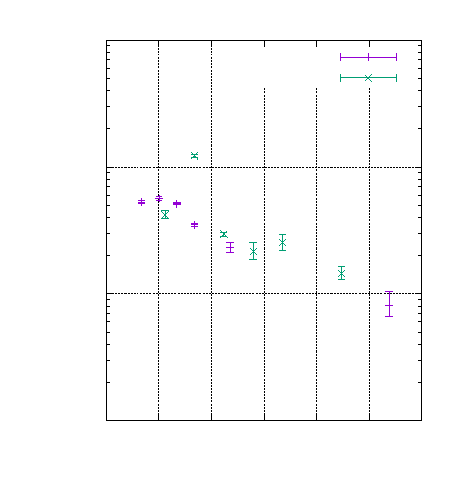
\includegraphics{cosktauconf}}%
    \gplfronttext
  \end{picture}%
\endgroup
\label{fig:cosconf}
    }
    \subfigure[][]{
    % GNUPLOT: LaTeX picture with Postscript
\begingroup
  \makeatletter
  \providecommand\color[2][]{%
    \GenericError{(gnuplot) \space\space\space\@spaces}{%
      Package color not loaded in conjunction with
      terminal option `colourtext'%
    }{See the gnuplot documentation for explanation.%
    }{Either use 'blacktext' in gnuplot or load the package
      color.sty in LaTeX.}%
    \renewcommand\color[2][]{}%
  }%
  \providecommand\includegraphics[2][]{%
    \GenericError{(gnuplot) \space\space\space\@spaces}{%
      Package graphicx or graphics not loaded%
    }{See the gnuplot documentation for explanation.%
    }{The gnuplot epslatex terminal needs graphicx.sty or graphics.sty.}%
    \renewcommand\includegraphics[2][]{}%
  }%
  \providecommand\rotatebox[2]{#2}%
  \@ifundefined{ifGPcolor}{%
    \newif\ifGPcolor
    \GPcolortrue
  }{}%
  \@ifundefined{ifGPblacktext}{%
    \newif\ifGPblacktext
    \GPblacktexttrue
  }{}%
  % define a \g@addto@macro without @ in the name:
  \let\gplgaddtomacro\g@addto@macro
  % define empty templates for all commands taking text:
  \gdef\gplbacktext{}%
  \gdef\gplfronttext{}%
  \makeatother
  \ifGPblacktext
    % no textcolor at all
    \def\colorrgb#1{}%
    \def\colorgray#1{}%
  \else
    % gray or color?
    \ifGPcolor
      \def\colorrgb#1{\color[rgb]{#1}}%
      \def\colorgray#1{\color[gray]{#1}}%
      \expandafter\def\csname LTw\endcsname{\color{white}}%
      \expandafter\def\csname LTb\endcsname{\color{black}}%
      \expandafter\def\csname LTa\endcsname{\color{black}}%
      \expandafter\def\csname LT0\endcsname{\color[rgb]{1,0,0}}%
      \expandafter\def\csname LT1\endcsname{\color[rgb]{0,1,0}}%
      \expandafter\def\csname LT2\endcsname{\color[rgb]{0,0,1}}%
      \expandafter\def\csname LT3\endcsname{\color[rgb]{1,0,1}}%
      \expandafter\def\csname LT4\endcsname{\color[rgb]{0,1,1}}%
      \expandafter\def\csname LT5\endcsname{\color[rgb]{1,1,0}}%
      \expandafter\def\csname LT6\endcsname{\color[rgb]{0,0,0}}%
      \expandafter\def\csname LT7\endcsname{\color[rgb]{1,0.3,0}}%
      \expandafter\def\csname LT8\endcsname{\color[rgb]{0.5,0.5,0.5}}%
    \else
      % gray
      \def\colorrgb#1{\color{black}}%
      \def\colorgray#1{\color[gray]{#1}}%
      \expandafter\def\csname LTw\endcsname{\color{white}}%
      \expandafter\def\csname LTb\endcsname{\color{black}}%
      \expandafter\def\csname LTa\endcsname{\color{black}}%
      \expandafter\def\csname LT0\endcsname{\color{black}}%
      \expandafter\def\csname LT1\endcsname{\color{black}}%
      \expandafter\def\csname LT2\endcsname{\color{black}}%
      \expandafter\def\csname LT3\endcsname{\color{black}}%
      \expandafter\def\csname LT4\endcsname{\color{black}}%
      \expandafter\def\csname LT5\endcsname{\color{black}}%
      \expandafter\def\csname LT6\endcsname{\color{black}}%
      \expandafter\def\csname LT7\endcsname{\color{black}}%
      \expandafter\def\csname LT8\endcsname{\color{black}}%
    \fi
  \fi
  \setlength{\unitlength}{0.0500bp}%
  \begin{picture}(4080.00,3400.00)%
    \gplgaddtomacro\gplbacktext{%
      \csname LTb\endcsname%
      \put(740,1058){\makebox(0,0)[r]{\strut{}1}}%
      \csname LTb\endcsname%
      \put(740,2109){\makebox(0,0)[r]{\strut{}10}}%
      \csname LTb\endcsname%
      \put(740,3159){\makebox(0,0)[r]{\strut{}100}}%
      \csname LTb\endcsname%
      \put(860,440){\makebox(0,0){\strut{}0}}%
      \csname LTb\endcsname%
      \put(1337,440){\makebox(0,0){\strut{}0.2}}%
      \csname LTb\endcsname%
      \put(1813,440){\makebox(0,0){\strut{}0.4}}%
      \csname LTb\endcsname%
      \put(2290,440){\makebox(0,0){\strut{}0.6}}%
      \csname LTb\endcsname%
      \put(2766,440){\makebox(0,0){\strut{}0.8}}%
      \csname LTb\endcsname%
      \put(3243,440){\makebox(0,0){\strut{}1}}%
      \csname LTb\endcsname%
      \put(3719,440){\makebox(0,0){\strut{}1.2}}%
      \put(160,1899){\rotatebox{-270}{\makebox(0,0){\strut{}$\tau$ /[s]}}}%
      \put(2289,140){\makebox(0,0){\strut{}$k$ /[$\micro$m$^{-1}$]}}%
    }%
    \gplgaddtomacro\gplfronttext{%
      \csname LTb\endcsname%
      \put(3128,2935){\makebox(0,0)[r]{\strut{}Fri sträng nr. 1}}%
      \csname LTb\endcsname%
      \put(3128,2735){\makebox(0,0)[r]{\strut{}Fri sträng nr. 2}}%
    }%
    \gplbacktext
    \put(0,0){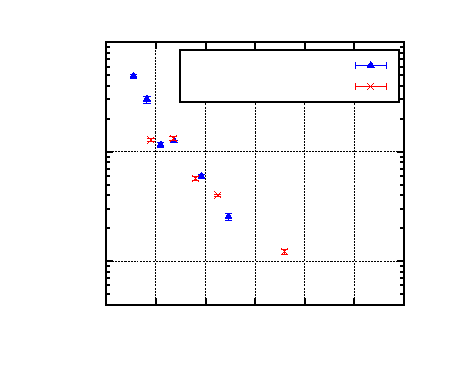
\includegraphics{cosktaunonconf}}%
    \gplfronttext
  \end{picture}%
\endgroup
\label{fig:cosnonconf}
    }}
    \caption{Samband mellan vågtal och relaxationstid för de första cosinusmoderna. Vardera figur innehåller data från 2 strängar för fria samt instängda strängar. För moder med större vågtal erhölls inget användbart samband, därför plottas enbart de signifikanta moderna för vardera sträng. Felmariginalerna för $\tau$ är satta som 95\,\%-iga konfidensintervall. Standardavvikelsen för $\tau$ fås som standardavvikelsen vid anpassningen av exponentialfunktionen.}
    \label{fig:cosmoder}
\end{figure}

Enligt \eqref{basutv} kan avståndsvektorn $A(t,s)$, innehållandes strängens transversella 
fluktuationer, uttryckas i en bas av egenmoder. Tidigare erhölls det att en sådan bas spänns upp av egenvektorerna $\psi_{n}(s)=\cos({\frac{n\pi}{L}s})$ vars fourierkoefficienter fås genom diskret cosinustransform av $A(t,s)$. Korrelationen för de tidsberoende koefficienterna beräknas enligt \eqref{modkorr} och modernas relaxationstid erhålls. I figur \ref{fig:cosmoder} (a) ses relaxationstider $\tau$ plottade mot modens vågtal $k$ för strängar inneslutna i en mikrokanal. Figur \ref{fig:cosmoder} (b) visar motsvarande data fast för de fria strängarna. Överensstämmande med \eqref{relaxconf} så ses ett snabbt avtagande samband för båda typerna av strängar, alltså att moder med små vågtal förblir representativa för strängens svängningar under längre tidsperioder.




\subsubsection{Strängarna kan representeras av egenmoder från kovariansmatrisen}

\begin{figure}
    \centering
    % GNUPLOT: LaTeX picture with Postscript
\begingroup
  \makeatletter
  \providecommand\color[2][]{%
    \GenericError{(gnuplot) \space\space\space\@spaces}{%
      Package color not loaded in conjunction with
      terminal option `colourtext'%
    }{See the gnuplot documentation for explanation.%
    }{Either use 'blacktext' in gnuplot or load the package
      color.sty in LaTeX.}%
    \renewcommand\color[2][]{}%
  }%
  \providecommand\includegraphics[2][]{%
    \GenericError{(gnuplot) \space\space\space\@spaces}{%
      Package graphicx or graphics not loaded%
    }{See the gnuplot documentation for explanation.%
    }{The gnuplot epslatex terminal needs graphicx.sty or graphics.sty.}%
    \renewcommand\includegraphics[2][]{}%
  }%
  \providecommand\rotatebox[2]{#2}%
  \@ifundefined{ifGPcolor}{%
    \newif\ifGPcolor
    \GPcolortrue
  }{}%
  \@ifundefined{ifGPblacktext}{%
    \newif\ifGPblacktext
    \GPblacktexttrue
  }{}%
  % define a \g@addto@macro without @ in the name:
  \let\gplgaddtomacro\g@addto@macro
  % define empty templates for all commands taking text:
  \gdef\gplbacktext{}%
  \gdef\gplfronttext{}%
  \makeatother
  \ifGPblacktext
    % no textcolor at all
    \def\colorrgb#1{}%
    \def\colorgray#1{}%
  \else
    % gray or color?
    \ifGPcolor
      \def\colorrgb#1{\color[rgb]{#1}}%
      \def\colorgray#1{\color[gray]{#1}}%
      \expandafter\def\csname LTw\endcsname{\color{white}}%
      \expandafter\def\csname LTb\endcsname{\color{black}}%
      \expandafter\def\csname LTa\endcsname{\color{black}}%
      \expandafter\def\csname LT0\endcsname{\color[rgb]{1,0,0}}%
      \expandafter\def\csname LT1\endcsname{\color[rgb]{0,1,0}}%
      \expandafter\def\csname LT2\endcsname{\color[rgb]{0,0,1}}%
      \expandafter\def\csname LT3\endcsname{\color[rgb]{1,0,1}}%
      \expandafter\def\csname LT4\endcsname{\color[rgb]{0,1,1}}%
      \expandafter\def\csname LT5\endcsname{\color[rgb]{1,1,0}}%
      \expandafter\def\csname LT6\endcsname{\color[rgb]{0,0,0}}%
      \expandafter\def\csname LT7\endcsname{\color[rgb]{1,0.3,0}}%
      \expandafter\def\csname LT8\endcsname{\color[rgb]{0.5,0.5,0.5}}%
    \else
      % gray
      \def\colorrgb#1{\color{black}}%
      \def\colorgray#1{\color[gray]{#1}}%
      \expandafter\def\csname LTw\endcsname{\color{white}}%
      \expandafter\def\csname LTb\endcsname{\color{black}}%
      \expandafter\def\csname LTa\endcsname{\color{black}}%
      \expandafter\def\csname LT0\endcsname{\color{black}}%
      \expandafter\def\csname LT1\endcsname{\color{black}}%
      \expandafter\def\csname LT2\endcsname{\color{black}}%
      \expandafter\def\csname LT3\endcsname{\color{black}}%
      \expandafter\def\csname LT4\endcsname{\color{black}}%
      \expandafter\def\csname LT5\endcsname{\color{black}}%
      \expandafter\def\csname LT6\endcsname{\color{black}}%
      \expandafter\def\csname LT7\endcsname{\color{black}}%
      \expandafter\def\csname LT8\endcsname{\color{black}}%
    \fi
  \fi
    \setlength{\unitlength}{0.0500bp}%
    \ifx\gptboxheight\undefined%
      \newlength{\gptboxheight}%
      \newlength{\gptboxwidth}%
      \newsavebox{\gptboxtext}%
    \fi%
    \setlength{\fboxrule}{0.5pt}%
    \setlength{\fboxsep}{1pt}%
\begin{picture}(6802.00,4534.00)%
    \gplgaddtomacro\gplbacktext{%
      \csname LTb\endcsname%
      \put(980,814){\makebox(0,0)[r]{\strut{}$10^{-29}$}}%
      \csname LTb\endcsname%
      \put(980,1510){\makebox(0,0)[r]{\strut{}$10^{-25}$}}%
      \csname LTb\endcsname%
      \put(980,2206){\makebox(0,0)[r]{\strut{}$10^{-21}$}}%
      \csname LTb\endcsname%
      \put(980,2901){\makebox(0,0)[r]{\strut{}$10^{-17}$}}%
      \csname LTb\endcsname%
      \put(980,3597){\makebox(0,0)[r]{\strut{}$10^{-13}$}}%
      \csname LTb\endcsname%
      \put(980,4293){\makebox(0,0)[r]{\strut{}$10^{-9}$}}%
      \csname LTb\endcsname%
      \put(1314,440){\makebox(0,0){\strut{}$20$}}%
      \csname LTb\endcsname%
      \put(2168,440){\makebox(0,0){\strut{}$40$}}%
      \csname LTb\endcsname%
      \put(3023,440){\makebox(0,0){\strut{}$60$}}%
      \csname LTb\endcsname%
      \put(3877,440){\makebox(0,0){\strut{}$80$}}%
      \csname LTb\endcsname%
      \put(4732,440){\makebox(0,0){\strut{}$100$}}%
      \csname LTb\endcsname%
      \put(5586,440){\makebox(0,0){\strut{}$120$}}%
      \csname LTb\endcsname%
      \put(6441,440){\makebox(0,0){\strut{}$140$}}%
    }%
    \gplgaddtomacro\gplfronttext{%
      \csname LTb\endcsname%
      \put(160,2466){\rotatebox{-270}{\makebox(0,0){\strut{}var[B$_i$]/[m$^2$]}}}%
      \put(3770,140){\makebox(0,0){\strut{}$\lambda_k$}}%
      \csname LTb\endcsname%
      \put(2480,4130){\makebox(0,0)[r]{\strut{}confined}}%
      \csname LTb\endcsname%
      \put(2480,3930){\makebox(0,0)[r]{\strut{}confined}}%
      \csname LTb\endcsname%
      \put(2480,3730){\makebox(0,0)[r]{\strut{}non-confined}}%
      \csname LTb\endcsname%
      \put(2480,3530){\makebox(0,0)[r]{\strut{}non-confined}}%
    }%
    \gplbacktext
    \put(0,0){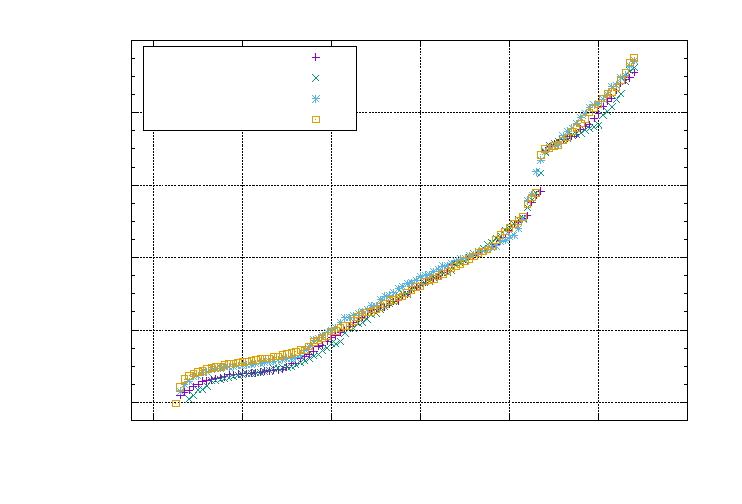
\includegraphics{kovegenv}}%
    \gplfronttext
  \end{picture}%
\endgroup

    \caption{De största egenvärdena till kovariansmatrisen från \eqref{eq:C} för de fyra strängarna som studerats. Det ses att $\VAR{\mathbf{B}_i}$ varierar stort då $\VAR{\mathbf{B}_1}/\VAR{\mathbf{B}_{20}}\approx10^7$. Icke visade egenvärden avtar exponentiellt och dessa moder bidrar inte signifikant till strängens rörelse.}
    \label{fig:kovegenvarde}
\end{figure}

\begin{figure}
    \centering
    % GNUPLOT: LaTeX picture with Postscript
\begingroup
  \makeatletter
  \providecommand\color[2][]{%
    \GenericError{(gnuplot) \space\space\space\@spaces}{%
      Package color not loaded in conjunction with
      terminal option `colourtext'%
    }{See the gnuplot documentation for explanation.%
    }{Either use 'blacktext' in gnuplot or load the package
      color.sty in LaTeX.}%
    \renewcommand\color[2][]{}%
  }%
  \providecommand\includegraphics[2][]{%
    \GenericError{(gnuplot) \space\space\space\@spaces}{%
      Package graphicx or graphics not loaded%
    }{See the gnuplot documentation for explanation.%
    }{The gnuplot epslatex terminal needs graphicx.sty or graphics.sty.}%
    \renewcommand\includegraphics[2][]{}%
  }%
  \providecommand\rotatebox[2]{#2}%
  \@ifundefined{ifGPcolor}{%
    \newif\ifGPcolor
    \GPcolortrue
  }{}%
  \@ifundefined{ifGPblacktext}{%
    \newif\ifGPblacktext
    \GPblacktexttrue
  }{}%
  % define a \g@addto@macro without @ in the name:
  \let\gplgaddtomacro\g@addto@macro
  % define empty templates for all commands taking text:
  \gdef\gplbacktext{}%
  \gdef\gplfronttext{}%
  \makeatother
  \ifGPblacktext
    % no textcolor at all
    \def\colorrgb#1{}%
    \def\colorgray#1{}%
  \else
    % gray or color?
    \ifGPcolor
      \def\colorrgb#1{\color[rgb]{#1}}%
      \def\colorgray#1{\color[gray]{#1}}%
      \expandafter\def\csname LTw\endcsname{\color{white}}%
      \expandafter\def\csname LTb\endcsname{\color{black}}%
      \expandafter\def\csname LTa\endcsname{\color{black}}%
      \expandafter\def\csname LT0\endcsname{\color[rgb]{1,0,0}}%
      \expandafter\def\csname LT1\endcsname{\color[rgb]{0,1,0}}%
      \expandafter\def\csname LT2\endcsname{\color[rgb]{0,0,1}}%
      \expandafter\def\csname LT3\endcsname{\color[rgb]{1,0,1}}%
      \expandafter\def\csname LT4\endcsname{\color[rgb]{0,1,1}}%
      \expandafter\def\csname LT5\endcsname{\color[rgb]{1,1,0}}%
      \expandafter\def\csname LT6\endcsname{\color[rgb]{0,0,0}}%
      \expandafter\def\csname LT7\endcsname{\color[rgb]{1,0.3,0}}%
      \expandafter\def\csname LT8\endcsname{\color[rgb]{0.5,0.5,0.5}}%
    \else
      % gray
      \def\colorrgb#1{\color{black}}%
      \def\colorgray#1{\color[gray]{#1}}%
      \expandafter\def\csname LTw\endcsname{\color{white}}%
      \expandafter\def\csname LTb\endcsname{\color{black}}%
      \expandafter\def\csname LTa\endcsname{\color{black}}%
      \expandafter\def\csname LT0\endcsname{\color{black}}%
      \expandafter\def\csname LT1\endcsname{\color{black}}%
      \expandafter\def\csname LT2\endcsname{\color{black}}%
      \expandafter\def\csname LT3\endcsname{\color{black}}%
      \expandafter\def\csname LT4\endcsname{\color{black}}%
      \expandafter\def\csname LT5\endcsname{\color{black}}%
      \expandafter\def\csname LT6\endcsname{\color{black}}%
      \expandafter\def\csname LT7\endcsname{\color{black}}%
      \expandafter\def\csname LT8\endcsname{\color{black}}%
    \fi
  \fi
    \setlength{\unitlength}{0.0500bp}%
    \ifx\gptboxheight\undefined%
      \newlength{\gptboxheight}%
      \newlength{\gptboxwidth}%
      \newsavebox{\gptboxtext}%
    \fi%
    \setlength{\fboxrule}{0.5pt}%
    \setlength{\fboxsep}{1pt}%
\begin{picture}(6802.00,3968.00)%
    \gplgaddtomacro\gplbacktext{%
      \csname LTb\endcsname%
      \put(980,640){\makebox(0,0)[r]{\strut{}$-0,15$}}%
      \csname LTb\endcsname%
      \put(980,1026){\makebox(0,0)[r]{\strut{}$-0,1$}}%
      \csname LTb\endcsname%
      \put(980,1412){\makebox(0,0)[r]{\strut{}$-0,05$}}%
      \csname LTb\endcsname%
      \put(980,1798){\makebox(0,0)[r]{\strut{}$0$}}%
      \csname LTb\endcsname%
      \put(980,2184){\makebox(0,0)[r]{\strut{}$0,05$}}%
      \csname LTb\endcsname%
      \put(980,2569){\makebox(0,0)[r]{\strut{}$0,1$}}%
      \csname LTb\endcsname%
      \put(980,2955){\makebox(0,0)[r]{\strut{}$0,15$}}%
      \csname LTb\endcsname%
      \put(980,3341){\makebox(0,0)[r]{\strut{}$0,2$}}%
      \csname LTb\endcsname%
      \put(980,3727){\makebox(0,0)[r]{\strut{}$0,25$}}%
      \csname LTb\endcsname%
      \put(1100,440){\makebox(0,0){\strut{}$0$}}%
      \csname LTb\endcsname%
      \put(1863,440){\makebox(0,0){\strut{}$5$}}%
      \csname LTb\endcsname%
      \put(2626,440){\makebox(0,0){\strut{}$10$}}%
      \csname LTb\endcsname%
      \put(3389,440){\makebox(0,0){\strut{}$15$}}%
      \csname LTb\endcsname%
      \put(4152,440){\makebox(0,0){\strut{}$20$}}%
      \csname LTb\endcsname%
      \put(4915,440){\makebox(0,0){\strut{}$25$}}%
      \csname LTb\endcsname%
      \put(5678,440){\makebox(0,0){\strut{}$30$}}%
      \csname LTb\endcsname%
      \put(6441,440){\makebox(0,0){\strut{}$35$}}%
    }%
    \gplgaddtomacro\gplfronttext{%
      \csname LTb\endcsname%
      \put(160,2183){\rotatebox{-270}{\makebox(0,0){\strut{}$v_i(l)$}}}%
      \put(3770,140){\makebox(0,0){\strut{}$l$ /[$\micro$m]}}%
      \csname LTb\endcsname%
      \put(2776,3514){\makebox(0,0)[r]{\strut{}$\mathbf{B}_2$}}%
      \csname LTb\endcsname%
      \put(3679,3514){\makebox(0,0)[r]{\strut{}$\mathbf{B}_3$}}%
      \csname LTb\endcsname%
      \put(4582,3514){\makebox(0,0)[r]{\strut{}$\mathbf{B}_4$}}%
    }%
    \gplbacktext
    \put(0,0){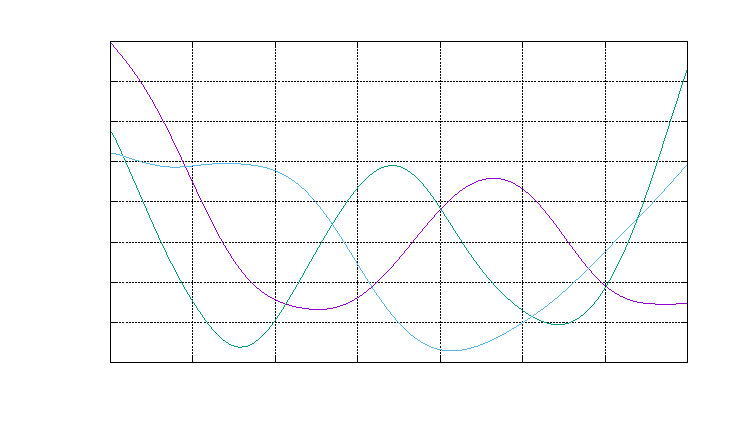
\includegraphics{moder}}%
    \gplfronttext
  \end{picture}%
\endgroup

    \caption{Typiska egenmoder för en sträng. Dessa egenmoder hör till en fri sträng men inga väsentliga skillnader för egenmodernas utseende fanns mellan fria och instängda strängar. Det ses att delar av egenmoderna liknar harmoniska svängningar; avvikelse från detta är störst vid ändarna på strängen.}
    \label{fig:egenmoder}
\end{figure}

\begin{figure}
    \centering
    % GNUPLOT: LaTeX picture with Postscript
\begingroup
  \makeatletter
  \providecommand\color[2][]{%
    \GenericError{(gnuplot) \space\space\space\@spaces}{%
      Package color not loaded in conjunction with
      terminal option `colourtext'%
    }{See the gnuplot documentation for explanation.%
    }{Either use 'blacktext' in gnuplot or load the package
      color.sty in LaTeX.}%
    \renewcommand\color[2][]{}%
  }%
  \providecommand\includegraphics[2][]{%
    \GenericError{(gnuplot) \space\space\space\@spaces}{%
      Package graphicx or graphics not loaded%
    }{See the gnuplot documentation for explanation.%
    }{The gnuplot epslatex terminal needs graphicx.sty or graphics.sty.}%
    \renewcommand\includegraphics[2][]{}%
  }%
  \providecommand\rotatebox[2]{#2}%
  \@ifundefined{ifGPcolor}{%
    \newif\ifGPcolor
    \GPcolortrue
  }{}%
  \@ifundefined{ifGPblacktext}{%
    \newif\ifGPblacktext
    \GPblacktexttrue
  }{}%
  % define a \g@addto@macro without @ in the name:
  \let\gplgaddtomacro\g@addto@macro
  % define empty templates for all commands taking text:
  \gdef\gplbacktext{}%
  \gdef\gplfronttext{}%
  \makeatother
  \ifGPblacktext
    % no textcolor at all
    \def\colorrgb#1{}%
    \def\colorgray#1{}%
  \else
    % gray or color?
    \ifGPcolor
      \def\colorrgb#1{\color[rgb]{#1}}%
      \def\colorgray#1{\color[gray]{#1}}%
      \expandafter\def\csname LTw\endcsname{\color{white}}%
      \expandafter\def\csname LTb\endcsname{\color{black}}%
      \expandafter\def\csname LTa\endcsname{\color{black}}%
      \expandafter\def\csname LT0\endcsname{\color[rgb]{1,0,0}}%
      \expandafter\def\csname LT1\endcsname{\color[rgb]{0,1,0}}%
      \expandafter\def\csname LT2\endcsname{\color[rgb]{0,0,1}}%
      \expandafter\def\csname LT3\endcsname{\color[rgb]{1,0,1}}%
      \expandafter\def\csname LT4\endcsname{\color[rgb]{0,1,1}}%
      \expandafter\def\csname LT5\endcsname{\color[rgb]{1,1,0}}%
      \expandafter\def\csname LT6\endcsname{\color[rgb]{0,0,0}}%
      \expandafter\def\csname LT7\endcsname{\color[rgb]{1,0.3,0}}%
      \expandafter\def\csname LT8\endcsname{\color[rgb]{0.5,0.5,0.5}}%
    \else
      % gray
      \def\colorrgb#1{\color{black}}%
      \def\colorgray#1{\color[gray]{#1}}%
      \expandafter\def\csname LTw\endcsname{\color{white}}%
      \expandafter\def\csname LTb\endcsname{\color{black}}%
      \expandafter\def\csname LTa\endcsname{\color{black}}%
      \expandafter\def\csname LT0\endcsname{\color{black}}%
      \expandafter\def\csname LT1\endcsname{\color{black}}%
      \expandafter\def\csname LT2\endcsname{\color{black}}%
      \expandafter\def\csname LT3\endcsname{\color{black}}%
      \expandafter\def\csname LT4\endcsname{\color{black}}%
      \expandafter\def\csname LT5\endcsname{\color{black}}%
      \expandafter\def\csname LT6\endcsname{\color{black}}%
      \expandafter\def\csname LT7\endcsname{\color{black}}%
      \expandafter\def\csname LT8\endcsname{\color{black}}%
    \fi
  \fi
    \setlength{\unitlength}{0.0500bp}%
    \ifx\gptboxheight\undefined%
      \newlength{\gptboxheight}%
      \newlength{\gptboxwidth}%
      \newsavebox{\gptboxtext}%
    \fi%
    \setlength{\fboxrule}{0.5pt}%
    \setlength{\fboxsep}{1pt}%
\begin{picture}(6802.00,3968.00)%
    \gplgaddtomacro\gplbacktext{%
      \csname LTb\endcsname%
      \put(980,640){\makebox(0,0)[r]{\strut{}$10^{-13}$}}%
      \csname LTb\endcsname%
      \put(980,1726){\makebox(0,0)[r]{\strut{}$10^{-12}$}}%
      \csname LTb\endcsname%
      \put(980,2812){\makebox(0,0)[r]{\strut{}$10^{-11}$}}%
      \csname LTb\endcsname%
      \put(1100,440){\makebox(0,0){\strut{}$0$}}%
      \csname LTb\endcsname%
      \put(2435,440){\makebox(0,0){\strut{}$0.5$}}%
      \csname LTb\endcsname%
      \put(3771,440){\makebox(0,0){\strut{}$1$}}%
      \csname LTb\endcsname%
      \put(5106,440){\makebox(0,0){\strut{}$1.5$}}%
      \csname LTb\endcsname%
      \put(6441,440){\makebox(0,0){\strut{}$2$}}%
    }%
    \gplgaddtomacro\gplfronttext{%
      \csname LTb\endcsname%
      \put(160,2183){\rotatebox{-270}{\makebox(0,0){\strut{}$\ev{B_{i}(t)B_{i}(t+\Delta t)}$}}}%
      \put(3770,140){\makebox(0,0){\strut{}$\Delta t$/[s]}}%
    }%
    \gplbacktext
    \put(0,0){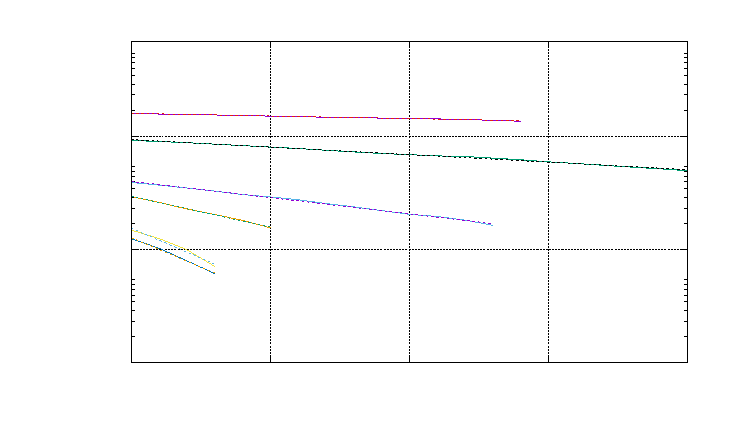
\includegraphics{korrfil3}}%
    \gplfronttext
  \end{picture}%
\endgroup

    \caption{Korrelationen \eqref{eq:korrmoder} för de sex egenmoderna med störst varians. Ett exponentiellt samband ses mellan korrelationen och tiden. En trendlinje anpassas i minsta-kvadrat mening och lutningen $a_i$ ger relaxationstiden enligt $\tau_i=\nicefrac{1}{\abs{a_i}}$. Relaxationstiderna för moderna ges i figuren.}
    \label{fig:korrelation}
\end{figure}

Egenvärdena, som är precis $\VAR{\mathbf{B}_i}$, till kovariansmatrisen bildad från de stokastiska processerna $A_s(t)$ visas i \figref{fig:kovegenvarde} och en tydlig spridning i storlek ses. Den stora skillnaden i varians visar att strängrörelsen till en god approximation kan beskrivas i ett fåtal egenmoder snarare än separata avstånd i varje punkt längs strängen. Vidare visas i \figref{fig:egenmoder} tre typiska egenmoder för strängarna vars egenmoder hör till en fri sträng. Ingen karakteristisk skillnad mellan egenmoderna för fria respektive instängda strängar verkade finnas. Egenmoderna liknar till viss grad harmoniska svängningar där den största avvikelsen ses vara vid strängens ändar.
%Antalet egenvärde \sim polynomgrad

Vidare bestäms en relaxationstid för varje strängs egenmoder enligt \eqref{eq:korrmoder}. Detta plottas i \figref{fig:korrelation} för en fri sträng vars första sex egenmoder studeras. Korrelationen ses följa ett exponentiellt samband väl och en relaxationstid $\tau$ beräknas. Relaxationstiderna för den fria strängen plottad i \figref{fig:korrelation} ses vara inom intervallet \unit[0,3--8,0]{s}. Då $\tau$ avtar med storleken på moden bestäms dessa endast för de största moderna, statistiken för moder med kortare relaxationstider är för liten. 

Eftersom egenmoderna beter sig harmoniskt uppskattas ett vågtal till vardera egenmod genom anpassning av en cosinusfunktion. Vågtalen för de fyra strängarna visas i \figref{fig:dispersion} där de plottas mot relaxationstiderna för motsvarande egenmod. Relaxationstiderna ses minska med ökat vågtal med en viss avvikelse för moder med lägst vågtal. De fria strängarnas relaxationstid är inom intervallet \unit[0,1--10]{s} och motsvarande för instängda strängar är \unit[0,1--2]{s}.

%Felgränsen på vågtalet tas fram genom att plotta egenmoden mot andraderivatan av den samma i \figref{fig:osak_vagtal}, för en exakt cosinusvåg väntas en rak linje med lutning $-k^2$; ty $\pd_x^2\cos{kx}=-k^2\cos{kx}$. Genom att anpassa en trendlinje i minsta kvadratmening och mäta standardavvikelsen för anpassningen kan en felgräns uppskattas, vilket används för att bestämma ett 95\, \% konfidensintervall. 

\begin{figure}\centerline{
\subfigure[][]{
% GNUPLOT: LaTeX picture with Postscript
\begingroup
  \makeatletter
  \providecommand\color[2][]{%
    \GenericError{(gnuplot) \space\space\space\@spaces}{%
      Package color not loaded in conjunction with
      terminal option `colourtext'%
    }{See the gnuplot documentation for explanation.%
    }{Either use 'blacktext' in gnuplot or load the package
      color.sty in LaTeX.}%
    \renewcommand\color[2][]{}%
  }%
  \providecommand\includegraphics[2][]{%
    \GenericError{(gnuplot) \space\space\space\@spaces}{%
      Package graphicx or graphics not loaded%
    }{See the gnuplot documentation for explanation.%
    }{The gnuplot epslatex terminal needs graphicx.sty or graphics.sty.}%
    \renewcommand\includegraphics[2][]{}%
  }%
  \providecommand\rotatebox[2]{#2}%
  \@ifundefined{ifGPcolor}{%
    \newif\ifGPcolor
    \GPcolortrue
  }{}%
  \@ifundefined{ifGPblacktext}{%
    \newif\ifGPblacktext
    \GPblacktexttrue
  }{}%
  % define a \g@addto@macro without @ in the name:
  \let\gplgaddtomacro\g@addto@macro
  % define empty templates for all commands taking text:
  \gdef\gplbacktext{}%
  \gdef\gplfronttext{}%
  \makeatother
  \ifGPblacktext
    % no textcolor at all
    \def\colorrgb#1{}%
    \def\colorgray#1{}%
  \else
    % gray or color?
    \ifGPcolor
      \def\colorrgb#1{\color[rgb]{#1}}%
      \def\colorgray#1{\color[gray]{#1}}%
      \expandafter\def\csname LTw\endcsname{\color{white}}%
      \expandafter\def\csname LTb\endcsname{\color{black}}%
      \expandafter\def\csname LTa\endcsname{\color{black}}%
      \expandafter\def\csname LT0\endcsname{\color[rgb]{1,0,0}}%
      \expandafter\def\csname LT1\endcsname{\color[rgb]{0,1,0}}%
      \expandafter\def\csname LT2\endcsname{\color[rgb]{0,0,1}}%
      \expandafter\def\csname LT3\endcsname{\color[rgb]{1,0,1}}%
      \expandafter\def\csname LT4\endcsname{\color[rgb]{0,1,1}}%
      \expandafter\def\csname LT5\endcsname{\color[rgb]{1,1,0}}%
      \expandafter\def\csname LT6\endcsname{\color[rgb]{0,0,0}}%
      \expandafter\def\csname LT7\endcsname{\color[rgb]{1,0.3,0}}%
      \expandafter\def\csname LT8\endcsname{\color[rgb]{0.5,0.5,0.5}}%
    \else
      % gray
      \def\colorrgb#1{\color{black}}%
      \def\colorgray#1{\color[gray]{#1}}%
      \expandafter\def\csname LTw\endcsname{\color{white}}%
      \expandafter\def\csname LTb\endcsname{\color{black}}%
      \expandafter\def\csname LTa\endcsname{\color{black}}%
      \expandafter\def\csname LT0\endcsname{\color{black}}%
      \expandafter\def\csname LT1\endcsname{\color{black}}%
      \expandafter\def\csname LT2\endcsname{\color{black}}%
      \expandafter\def\csname LT3\endcsname{\color{black}}%
      \expandafter\def\csname LT4\endcsname{\color{black}}%
      \expandafter\def\csname LT5\endcsname{\color{black}}%
      \expandafter\def\csname LT6\endcsname{\color{black}}%
      \expandafter\def\csname LT7\endcsname{\color{black}}%
      \expandafter\def\csname LT8\endcsname{\color{black}}%
    \fi
  \fi
    \setlength{\unitlength}{0.0500bp}%
    \ifx\gptboxheight\undefined%
      \newlength{\gptboxheight}%
      \newlength{\gptboxwidth}%
      \newsavebox{\gptboxtext}%
    \fi%
    \setlength{\fboxrule}{0.5pt}%
    \setlength{\fboxsep}{1pt}%
\begin{picture}(4250.00,4534.00)%
    \gplgaddtomacro\gplbacktext{%
      \csname LTb\endcsname%
      \put(740,640){\makebox(0,0)[r]{\strut{}0.1}}%
      \csname LTb\endcsname%
      \put(740,2467){\makebox(0,0)[r]{\strut{}1}}%
      \csname LTb\endcsname%
      \put(740,4293){\makebox(0,0)[r]{\strut{}10}}%
      \csname LTb\endcsname%
      \put(860,440){\makebox(0,0){\strut{}0}}%
      \csname LTb\endcsname%
      \put(1466,440){\makebox(0,0){\strut{}0.2}}%
      \csname LTb\endcsname%
      \put(2072,440){\makebox(0,0){\strut{}0.4}}%
      \csname LTb\endcsname%
      \put(2677,440){\makebox(0,0){\strut{}0.6}}%
      \csname LTb\endcsname%
      \put(3283,440){\makebox(0,0){\strut{}0.8}}%
      \csname LTb\endcsname%
      \put(3889,440){\makebox(0,0){\strut{}1}}%
    }%
    \gplgaddtomacro\gplfronttext{%
      \csname LTb\endcsname%
      \put(160,2466){\rotatebox{-270}{\makebox(0,0){\strut{}$\tau$/[s]}}}%
      \put(2374,140){\makebox(0,0){\strut{}$k$/[$\micro$m$^{-1}$]}}%
      \csname LTb\endcsname%
      \put(2986,4130){\makebox(0,0)[r]{\strut{}confined}}%
      \csname LTb\endcsname%
      \put(2986,3930){\makebox(0,0)[r]{\strut{}confined}}%
    }%
    \gplbacktext
    \put(0,0){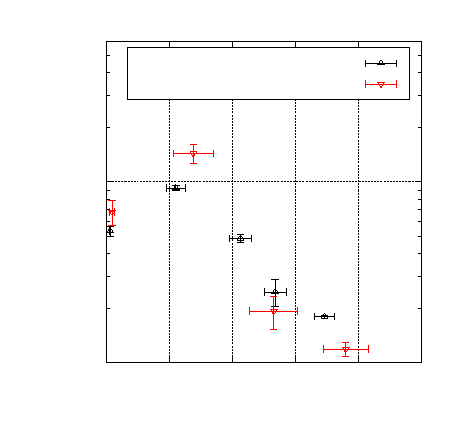
\includegraphics{ktauconf}}%
    \gplfronttext
  \end{picture}%
\endgroup
\label{fig:ktauconf}
}
\subfigure[][]{
% GNUPLOT: LaTeX picture with Postscript
\begingroup
  \makeatletter
  \providecommand\color[2][]{%
    \GenericError{(gnuplot) \space\space\space\@spaces}{%
      Package color not loaded in conjunction with
      terminal option `colourtext'%
    }{See the gnuplot documentation for explanation.%
    }{Either use 'blacktext' in gnuplot or load the package
      color.sty in LaTeX.}%
    \renewcommand\color[2][]{}%
  }%
  \providecommand\includegraphics[2][]{%
    \GenericError{(gnuplot) \space\space\space\@spaces}{%
      Package graphicx or graphics not loaded%
    }{See the gnuplot documentation for explanation.%
    }{The gnuplot epslatex terminal needs graphicx.sty or graphics.sty.}%
    \renewcommand\includegraphics[2][]{}%
  }%
  \providecommand\rotatebox[2]{#2}%
  \@ifundefined{ifGPcolor}{%
    \newif\ifGPcolor
    \GPcolortrue
  }{}%
  \@ifundefined{ifGPblacktext}{%
    \newif\ifGPblacktext
    \GPblacktexttrue
  }{}%
  % define a \g@addto@macro without @ in the name:
  \let\gplgaddtomacro\g@addto@macro
  % define empty templates for all commands taking text:
  \gdef\gplbacktext{}%
  \gdef\gplfronttext{}%
  \makeatother
  \ifGPblacktext
    % no textcolor at all
    \def\colorrgb#1{}%
    \def\colorgray#1{}%
  \else
    % gray or color?
    \ifGPcolor
      \def\colorrgb#1{\color[rgb]{#1}}%
      \def\colorgray#1{\color[gray]{#1}}%
      \expandafter\def\csname LTw\endcsname{\color{white}}%
      \expandafter\def\csname LTb\endcsname{\color{black}}%
      \expandafter\def\csname LTa\endcsname{\color{black}}%
      \expandafter\def\csname LT0\endcsname{\color[rgb]{1,0,0}}%
      \expandafter\def\csname LT1\endcsname{\color[rgb]{0,1,0}}%
      \expandafter\def\csname LT2\endcsname{\color[rgb]{0,0,1}}%
      \expandafter\def\csname LT3\endcsname{\color[rgb]{1,0,1}}%
      \expandafter\def\csname LT4\endcsname{\color[rgb]{0,1,1}}%
      \expandafter\def\csname LT5\endcsname{\color[rgb]{1,1,0}}%
      \expandafter\def\csname LT6\endcsname{\color[rgb]{0,0,0}}%
      \expandafter\def\csname LT7\endcsname{\color[rgb]{1,0.3,0}}%
      \expandafter\def\csname LT8\endcsname{\color[rgb]{0.5,0.5,0.5}}%
    \else
      % gray
      \def\colorrgb#1{\color{black}}%
      \def\colorgray#1{\color[gray]{#1}}%
      \expandafter\def\csname LTw\endcsname{\color{white}}%
      \expandafter\def\csname LTb\endcsname{\color{black}}%
      \expandafter\def\csname LTa\endcsname{\color{black}}%
      \expandafter\def\csname LT0\endcsname{\color{black}}%
      \expandafter\def\csname LT1\endcsname{\color{black}}%
      \expandafter\def\csname LT2\endcsname{\color{black}}%
      \expandafter\def\csname LT3\endcsname{\color{black}}%
      \expandafter\def\csname LT4\endcsname{\color{black}}%
      \expandafter\def\csname LT5\endcsname{\color{black}}%
      \expandafter\def\csname LT6\endcsname{\color{black}}%
      \expandafter\def\csname LT7\endcsname{\color{black}}%
      \expandafter\def\csname LT8\endcsname{\color{black}}%
    \fi
  \fi
    \setlength{\unitlength}{0.0500bp}%
    \ifx\gptboxheight\undefined%
      \newlength{\gptboxheight}%
      \newlength{\gptboxwidth}%
      \newsavebox{\gptboxtext}%
    \fi%
    \setlength{\fboxrule}{0.5pt}%
    \setlength{\fboxsep}{1pt}%
\begin{picture}(4250.00,3968.00)%
    \gplgaddtomacro\gplbacktext{%
      \csname LTb\endcsname%
      \put(740,640){\makebox(0,0)[r]{\strut{}0,1}}%
      \csname LTb\endcsname%
      \put(740,1918){\makebox(0,0)[r]{\strut{}1}}%
      \csname LTb\endcsname%
      \put(740,3197){\makebox(0,0)[r]{\strut{}10}}%
      \csname LTb\endcsname%
      \put(860,440){\makebox(0,0){\strut{}0}}%
      \csname LTb\endcsname%
      \put(1365,440){\makebox(0,0){\strut{}0,1}}%
      \csname LTb\endcsname%
      \put(1870,440){\makebox(0,0){\strut{}0,2}}%
      \csname LTb\endcsname%
      \put(2375,440){\makebox(0,0){\strut{}0,3}}%
      \csname LTb\endcsname%
      \put(2879,440){\makebox(0,0){\strut{}0,4}}%
      \csname LTb\endcsname%
      \put(3384,440){\makebox(0,0){\strut{}0,5}}%
      \csname LTb\endcsname%
      \put(3889,440){\makebox(0,0){\strut{}0,6}}%
    }%
    \gplgaddtomacro\gplfronttext{%
      \csname LTb\endcsname%
      \put(160,2183){\rotatebox{-270}{\makebox(0,0){\strut{}$\tau$ /[s]}}}%
      \put(2374,140){\makebox(0,0){\strut{}$k$ /[$\micro$m$^{-1}$]}}%
      \csname LTb\endcsname%
      \put(3226,3514){\makebox(0,0)[r]{\strut{}Fri sträng nr. 1}}%
      \csname LTb\endcsname%
      \put(3226,3314){\makebox(0,0)[r]{\strut{}Fri sträng nr. 2}}%
    }%
    \gplbacktext
    \put(0,0){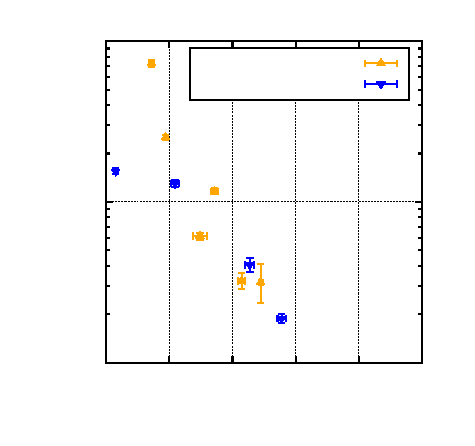
\includegraphics{ktaunonconf}}%
    \gplfronttext
  \end{picture}%
\endgroup
\label{fig:ktaunonconf}
}}
\caption{Relation mellan vågtal och relaxationstid för strängarnas egenmoder härledda från kovariansmatrisen. Bortsett från vissa moder med lågt $k$ så minskar relaxationstiden med ökande vågtal. Felmarginalerna för $\tau$ och $k$ är satta som 95\,\%-iga konfidensintervall. För $\tau$ används standardavvikelsen som fås vid anpassningen av exponentialfunktionen. Standardavvikelsen för $k$ beräknas genom att plotta egenmoden mot dess andraderivata. För en cosinusfunktion förväntas då ett linjärt samband med lutning $-k^2$, avvikelser från detta ger ett mått på egenmodens avvikelse från en cosinusfunktion.}
\label{fig:dispersion}
\end{figure}

%%%%%%%%%%%%%%%%%%%%%%%%%%%%%%%%%%%%%%%%%%%%%%%%%%%%%%%%%%%%%%%%%%%%%%%%%%%
\begin{comment}
\begin{figure}
    \centering
    % GNUPLOT: LaTeX picture with Postscript
\begingroup
  \makeatletter
  \providecommand\color[2][]{%
    \GenericError{(gnuplot) \space\space\space\@spaces}{%
      Package color not loaded in conjunction with
      terminal option `colourtext'%
    }{See the gnuplot documentation for explanation.%
    }{Either use 'blacktext' in gnuplot or load the package
      color.sty in LaTeX.}%
    \renewcommand\color[2][]{}%
  }%
  \providecommand\includegraphics[2][]{%
    \GenericError{(gnuplot) \space\space\space\@spaces}{%
      Package graphicx or graphics not loaded%
    }{See the gnuplot documentation for explanation.%
    }{The gnuplot epslatex terminal needs graphicx.sty or graphics.sty.}%
    \renewcommand\includegraphics[2][]{}%
  }%
  \providecommand\rotatebox[2]{#2}%
  \@ifundefined{ifGPcolor}{%
    \newif\ifGPcolor
    \GPcolortrue
  }{}%
  \@ifundefined{ifGPblacktext}{%
    \newif\ifGPblacktext
    \GPblacktexttrue
  }{}%
  % define a \g@addto@macro without @ in the name:
  \let\gplgaddtomacro\g@addto@macro
  % define empty templates for all commands taking text:
  \gdef\gplbacktext{}%
  \gdef\gplfronttext{}%
  \makeatother
  \ifGPblacktext
    % no textcolor at all
    \def\colorrgb#1{}%
    \def\colorgray#1{}%
  \else
    % gray or color?
    \ifGPcolor
      \def\colorrgb#1{\color[rgb]{#1}}%
      \def\colorgray#1{\color[gray]{#1}}%
      \expandafter\def\csname LTw\endcsname{\color{white}}%
      \expandafter\def\csname LTb\endcsname{\color{black}}%
      \expandafter\def\csname LTa\endcsname{\color{black}}%
      \expandafter\def\csname LT0\endcsname{\color[rgb]{1,0,0}}%
      \expandafter\def\csname LT1\endcsname{\color[rgb]{0,1,0}}%
      \expandafter\def\csname LT2\endcsname{\color[rgb]{0,0,1}}%
      \expandafter\def\csname LT3\endcsname{\color[rgb]{1,0,1}}%
      \expandafter\def\csname LT4\endcsname{\color[rgb]{0,1,1}}%
      \expandafter\def\csname LT5\endcsname{\color[rgb]{1,1,0}}%
      \expandafter\def\csname LT6\endcsname{\color[rgb]{0,0,0}}%
      \expandafter\def\csname LT7\endcsname{\color[rgb]{1,0.3,0}}%
      \expandafter\def\csname LT8\endcsname{\color[rgb]{0.5,0.5,0.5}}%
    \else
      % gray
      \def\colorrgb#1{\color{black}}%
      \def\colorgray#1{\color[gray]{#1}}%
      \expandafter\def\csname LTw\endcsname{\color{white}}%
      \expandafter\def\csname LTb\endcsname{\color{black}}%
      \expandafter\def\csname LTa\endcsname{\color{black}}%
      \expandafter\def\csname LT0\endcsname{\color{black}}%
      \expandafter\def\csname LT1\endcsname{\color{black}}%
      \expandafter\def\csname LT2\endcsname{\color{black}}%
      \expandafter\def\csname LT3\endcsname{\color{black}}%
      \expandafter\def\csname LT4\endcsname{\color{black}}%
      \expandafter\def\csname LT5\endcsname{\color{black}}%
      \expandafter\def\csname LT6\endcsname{\color{black}}%
      \expandafter\def\csname LT7\endcsname{\color{black}}%
      \expandafter\def\csname LT8\endcsname{\color{black}}%
    \fi
  \fi
    \setlength{\unitlength}{0.0500bp}%
    \ifx\gptboxheight\undefined%
      \newlength{\gptboxheight}%
      \newlength{\gptboxwidth}%
      \newsavebox{\gptboxtext}%
    \fi%
    \setlength{\fboxrule}{0.5pt}%
    \setlength{\fboxsep}{1pt}%
\begin{picture}(6802.00,3968.00)%
    \gplgaddtomacro\gplbacktext{%
      \csname LTb\endcsname%
      \put(980,640){\makebox(0,0)[r]{\strut{}$-0,04$}}%
      \csname LTb\endcsname%
      \put(980,1026){\makebox(0,0)[r]{\strut{}$-0,03$}}%
      \csname LTb\endcsname%
      \put(980,1412){\makebox(0,0)[r]{\strut{}$-0,02$}}%
      \csname LTb\endcsname%
      \put(980,1798){\makebox(0,0)[r]{\strut{}$-0,01$}}%
      \csname LTb\endcsname%
      \put(980,2184){\makebox(0,0)[r]{\strut{}$0$}}%
      \csname LTb\endcsname%
      \put(980,2569){\makebox(0,0)[r]{\strut{}$0,01$}}%
      \csname LTb\endcsname%
      \put(980,2955){\makebox(0,0)[r]{\strut{}$0,02$}}%
      \csname LTb\endcsname%
      \put(980,3341){\makebox(0,0)[r]{\strut{}$0,03$}}%
      \csname LTb\endcsname%
      \put(980,3727){\makebox(0,0)[r]{\strut{}$0,04$}}%
      \csname LTb\endcsname%
      \put(1100,440){\makebox(0,0){\strut{}$-0,15$}}%
      \csname LTb\endcsname%
      \put(1863,440){\makebox(0,0){\strut{}$-0,1$}}%
      \csname LTb\endcsname%
      \put(2626,440){\makebox(0,0){\strut{}$-0,05$}}%
      \csname LTb\endcsname%
      \put(3389,440){\makebox(0,0){\strut{}$0$}}%
      \csname LTb\endcsname%
      \put(4152,440){\makebox(0,0){\strut{}$0,05$}}%
      \csname LTb\endcsname%
      \put(4915,440){\makebox(0,0){\strut{}$0,1$}}%
      \csname LTb\endcsname%
      \put(5678,440){\makebox(0,0){\strut{}$0,15$}}%
      \csname LTb\endcsname%
      \put(6441,440){\makebox(0,0){\strut{}$0,2$}}%
    }%
    \gplgaddtomacro\gplfronttext{%
      \csname LTb\endcsname%
      \put(160,2183){\rotatebox{-270}{\makebox(0,0){\strut{}$\frac{\pd^2 v_{i}}{\pd l^2}$ /[$\micro$m$^{-2}$]}}}%
      \put(3770,140){\makebox(0,0){\strut{}$v_i$}}%
    }%
    \gplbacktext
    \put(0,0){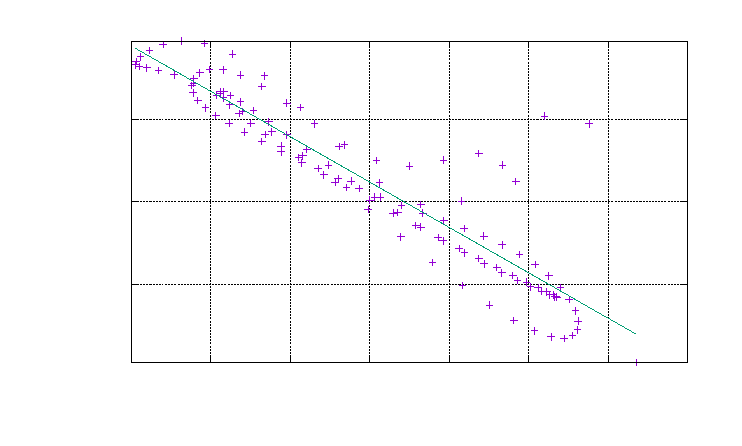
\includegraphics{osak_vagtal}}%
    \gplfronttext
  \end{picture}%
\endgroup

    \caption{Samband mellan $v_i(l)$ och $\frac{\pd^2v_i (l)}{\pd l^2}$ för att bestämma osäkerheten i anpassat vågtal. För en egenmod som är en exakt cosinusvåg väntas en rak linje med lutning $-k^2$; avvikelserna från en sådan linje antyder om hur mycket egenmoden avviker från en cosinusvåg.}
    \label{fig:osak_vagtal}
\end{figure}
\end{comment}
%%%%%%%%%%%%%%%%%%%%%%%%%%%%%%%%%%%%%%%%%%%%%%%%%%%%%%%%%%%%%%%%%%%%%%%%%%%


\section{Diskussion}

Strängrörelse är, på grund av stora svårigheter att avbilda små filament, mindre utforskad än partikelrörelser. Att strängar, till skillnad från partiklar, inte enbart kan beskrivas med en rumskoordinat gör dessutom en teoretisk analys mer krävande. Sammantaget kan man säga att strängstudierna har utgått från en mindre utbyggd flora av modeller än för partiklarna. Med detta i åtanke har denna studie ändå kunnat presentera vissa betänkliga resultat samt intressanta analyser och hypoteser.

Tyvärr har det statistiska underlaget för dessa studier varit väldigt tunt. Det studerade datamaterialet bestod enbart av fyra olika strängar, två fria och två instängda, med varierande längd. Detta gör att statistiska analyser riskerar att bli svagt underbyggda.
Dock bör det ändå påpekas att det för varje sträng finns omkring 100 datapunkter i vart och ett av cirka 100--300 tidsögonblick. Detta gör att det går att göra statistiska undersökningar för varje enskild sträng.


\subsection{Polynomanpassningens påverkan på resultatet}
%\todo[color=red,inline]{kort del om detta under egenmoder från kovariansmatrisen. se till så att det inte blir dubbelt.}

För att effektivt kunna studera strängens beteende gjordes en polynomanpassning till de pixlar som i varje bild representerade strängen. Det finns redan en motivering till detta val i avsnitt~\ref{sec:polynomanpassning}. Det här avsnittet kommer istället att fokusera på eventuella konsekvenser av polynomanpassningen och alternativa metoder som hade kunnat användas. 

En av dess konsekvenser är att gradtalet på polynomet påverkar hur många signifikanta egenmoder som kan detekteras. Som man kan se i \figref{fig:kovegenvarde} så gör egenvärdena en tydligt hopp efter omkring de 20 första. Att det är just efter de 20 första egenvärdena återfås oavsett hur många punkter strängen undersöks i. 
Detta visar sig faktiskt uppstå på grund av att polynomanpassningarna gjorts med 20-gradspolynom. 

Testar man med gradtal mellan 10 och 50 finner man för just dessa egenvärden att var detta hopp ligger beror på gradtalet. Dessutom blir hoppet mycket tydligare ju lägre gradtal som används. Och för de stora gradtalen minskar hoppet till att nästa inte gå att upptäcka vid grad 50. Det sistnämnda är lite märkligt, men skulle kunna orsakas av algoritmen för beräkning av egenvärden som MATLAB använder sig av.

%Eventuellt skulle även polynomen vara orsak till den något förhöjda tangentkorrelationen för små värden på $\Delta{s}$.\todo[color=cyan]{Vill vi säga något här, eller ska vi strunta i detta?}

\subsubsection{Alternativa metoder för att anpassa en kurva till strängdata}

I \figref{fig:strang_anpassning} kan man, utöver polynomanpassningen, även se en kubisk splineinterpolation. Detta är också ett sätt som använts för att anpassa en kurva till strängen~\cite{Koster_etal2005,Koster_etal2007}. Dock anser vi att beteendet som splineinterpolationen uppvisar i \figref{fig:strang_anpassning} inte speglar den verkliga strängens form. Det är inte särskilt troligt att den verkliga strängen helt skulle följa varje pixel, utan det är mer rimligt att den verkliga strängen följer en sorts medelposition av pixlarna. Detta eftersom det troligtvis finns brus i datan och att varje strängposition anges som den närmast belägna pixeln. Båda bidrar till att datan inte exakt representerar strängens form, åtminstone på liten längdskala.

En sak som ytterligare talar för att splineinterpolation inte är en optimal anpassningsmetod är svängningarna %\footnotemark{} 
som syns i \figref{fig:strang_anpassning} mellan pixlarna. Dessa svängningar sker över längdskalor som är mindre än mikroskopets upplösning. Det är alltså inte motiverat att använda sig av en metod som ger information på en längdskala som inte går att observera. 
%\footnotetext{Dessa svängningar är dock inte ett exempel på Runges fenomen. Eftersom en kubisk spline är flera olika tredjegradspolynom fås inte beteendet från ett höggradigt polynom\cite{Gustafsson_LaNa}. }



%\subsection{Strängen verkar vibrera kring ett jämviktläge}

%\subsection{Skillnad mellan fria och instängda strängar}
%Den tydligaste skillnaden mellan fria och instängda strängar är skillnaden i relaxationstiden för de olika egenmoderna vilket visades i \figref{fig:dispersion}. Att relaxationstiden för de fria strängarna spänner över ett större intervall anses rimligt, detta eftersom de är just fria; de begränsas inte av en kanal vilket torde göra att dess form är mer beständig i tiden.  



\subsection{Strängarna är styva med korrelerade tangentvektorer}

Datan som analyserades bestod av bildsekvenser på fria och begränsade aktinfilament. Då deras fluktuationer beskrivs som stokastiska har den statistiska analysen av filamenten främst behandlat rumsliga och temporala korrelationer. 

Resultaten visar att parametern persistence length, som ger ett mått på den längdskala under vilket filamentet kan anses vara styvt, är betydligt längre än filamentens längd. Då man behandlar de fritt fluktuerande filamenten underlättar det dataanalysen väsentligt. Detta då mer invecklade strängformer inte är möjliga; filamenten är därför huvudsakligen raka. Speciellt medför en lång persistence length att strängen inte viker över sig själv. 

%Dock försvåras analysen av tangentkorrelationer samt hur en mikrokanal påverkar strängars beteende. \todo{Förstår inte riktigt sista meningen.}

Då tangenkorrelationen beräknas ur WLC-modellen fås att tangentkorrelationen avtar exponentiellt. Dock ses i \figref{fig:tangentkorr} att tangentkorrelationen verkar innefatta någon form av tröghet för små längder. En förklaring hade varit att denna längdskala omfattar längden av enstaka aktinmolekyler. De kan då liknas vid en cykelkedja som har en minsta längd som går att böja. Så är dock inte fallet då denna längd är mycket större än enstaka aktinmolekyler. Istället kan det tänkas att det är strängarnas styvhet som ligger bakom fenomenet.  

Mikrokanalerna införs delvis för att fixera strängen längs en axel och studera om kanalen och strängen interagerar likt en mjuk potential. Mikrokanalens påverkan på strängen är en första approximation för att simulera så kallad \emph{macromolecular crowding}, som innebär att cellens inre komplexa struktur begränsar rörligheten inom cellen. Denna effekt gör att studier av biologiska fenomen inom respektive utanför cellen kan uppvisa signfikanta skillnader. 

För de strängar som undersöktes i denna rapport erhölls $L_{p}\gg L$, vars jämviktslägen grovt kan approximeras vara fixerade längs en axel. Det noterades ingen markant skillnad på strängens beteende då denna begränsas av en mikrokanal.
Därvid spekuleras att för en sträng med egenskaperna $L\gg L_{p}$, vars jämviktsläge vore mer intrasslat, skulle fixering i en mikrokanal markant påverka dess egenskaper. Alltså hade troligtvis dynamiken mellan mikrokanal och sträng blivit mer signifikant för längre strängar än för de i den här studien.

Dessa spekulationer tar stöd i modeller som utvecklas specifikt för tangenkorrelationen hos strängar i mikrokanaler. Där används parametern \emph{deflection length} $\lambda$ som definieras som kvoten mellan böjningsenergin och den paraboliska potentialen. Denna ger ett mått på den karakteristiska längd efter vilket en instängd sträng börjar återkorrelera. Enligt \cite{Koster_etal2007} fås att
\begin{equation}
\ev{\cos(\theta(\Delta s))}=1-\ev{\partial_{s}A(s)^2}=1-\frac{\lambda}{4L_\text{p}}
\qcomma \text{i gränsen då } s\to\infty.
\end{equation}
Vilket, i överensstämmelse med \figref{fig:tangentkorr}, ger att tangentkorrelationen för en sträng i en mikrokanal konvergerar mot ett positivt konstant värde. %Däremot erhölls även ett positivt värde för de fria strängarna. Då det inte kan förklaras av en yttre potential kan det orsakats av strängarnas struktur, eftersom skalärprodukten av tangentvektorer längs en rak sträng är alltid positiv.

%Vad som inte ses i \figref{fig:tangenkorr} är att även de asymptotiska korrelationerna för fria strängarna konvergerar mot ett konstant värde. Då det inte kan förklaras av en yttre potential kan det orsakas av strängarnas stavlika formation, skalärprodukten av tangentvektorerna längs en stav är alltid positiv.\todo{stavlika?}


%Dessa spekulationer tar stöd hos de modeller som utvecklas specifikt för tangenkorrelation hos strängar i mikrokanaler.   Modeller för att förklara detta beteende introducerar parametern \emph{deflection length} $\lambda$ vilket likt $L_\text{p}$ definieras som kvoten mellan böjningsenergin och den paraboliska potentialen. Enligt \cite{Koster_etal2007} fås den asymptotiska korrelationen som
%\begin{equation}
%\ev{\cos(\theta(\Delta s))}=1-\ev{\partial_{s}z(s)^2}=1-\frac{\lambda}{4L_\text{p}},
%\end{equation}
%vilket i överensstämmelse med \ref{fig:tangentkorr} ger att tangentkorrelationen konvergerar mot ett konstant värde. 
%\todo{Kolla över detta stycke}


\subsection{Kovariansmatrisen skulle kunna ge information om en ny modell för strängrörelsen}
Att variansen för egenmoderna framtagna från kovariansmatrisen sprider sig över ett stort intervall ($10^7$ för de $20$ största) indikerar att strängens rörelse till en god approximation kan representeras av okorrelerade egenmoder. 

Däremot verkar det finnas en koppling mellan antalet egenmoder med signifikant varians och gradtalet på de till strängarna anpassade polynomen. Så en för stor vikt ska inte läggas på det specifika antalet dominerande egenmoder. Även inom dessa $20$ största egenmoder så ska det noteras att bara ett fåtal av dessa har kunnat analyseras; exempelvis maximalt $7$ stycken för beräkning av vågtal samt relaxationstid. Valet av polynomgraden anses därför ha en liten inverkan på de presenterade resultaten.


\subsubsection{Egenmodsutvecklingen från kovariansmatrisen skulle kunna ge ledtrådar om en eventuell modell för strängarnas svängningar}
\label{disk:kovmatris}
Liknelsen mellan koefficienterna $b_i(t)$ med fourierkoefficienter i \eqref{eq:egenmoder_fourierkoef} är intressant. Den kan tyda på att egenvektorerna $\mathbf{B}_i$ skulle kunna översättas till en uppsättning basfunktioner $B_i(s)$ som beskriver strängens svängning. 
Jämför man detta med analysen i avsnitt~\ref{sec:costransform} och samtidigt betraktar likheten till svängningar i \figref{fig:egenmoder}, så väcks tanken på om det inte finns någon koppling mellan dem.

En möjlig tanke är att det skulle kunna gå att  koppla de uppmätta koefficienterna och egenfunktionerna till en styrande differentialekvation. Detta skulle dock kräva en mycket djupare teoretisk analys av kovariansmatrisen. %och dess koppling till en eventuell differentialekvation. 
Det är dock något som faller utanför denna studies räckvidd.
Vi har i dagsläget inte funnit några publicerade resultat som kan ge en klar teoretisk bild om det över huvud taget går att koppla kovariansmatrisens egenvektorer till en eventuell styrande differentialekvation. Likheterna som nämndes ovan skulle dock kunna tyda på att det är möjligt.
En sådan här koppling, om den finns, skulle kunna tillämpas som en statistiskt verktyg för att vidare undersöka strängrörelser.

Avslutningsvis bör vi påminna om att detta bara är spekulationer. Det verkar finnas vissa likheter, men utöver det så finns inga solida teoretiska grunder. Dock vill vi ändå mena att det vore intressant att vidare försöka studera kovariansmatrisens teoretiska egenskaper. Då särskilt om huruvida man kan göra en övergång från ändligtdimensionella vektorrum till ett funktionsrum i syfte att studera dess egenvektorer. 

\subsection{Cosinustransform respektive utveckling i egenmoder från kovariansmatrisen}
%Varför avviker egenmoder från kovmatris från cosvågor. Kan tänkas bero på att strängarnas fluktationer inte är homogen, mer svängning vid de lösa ändarna. 
%Anledningen till att studera strängens rörelse både genom cosinustranform samt egenmoder framtagna från kovariansmatrisen var huvudsakligen av två skäl. Cosinustransformens fördel är att vågtalen för cosinusbasen är exakt bestämda. Detta till skillnad mot egenmoderna från kovariansmatrisen vars form enligt tidigare ej nödvändigtvis behöver likna cosinusfunktioner vilket skulle kunna komplicera beräkning av vågtalet. \todo{ngt mer här}

%Fördelen med att använda egenmoderna framtagna från kovariansmatrisen är att variansen av egenmoderna ger ett mått på hur mycket av rörelsen som representeras av just den egenmoden. Därför kan karakteristiska egenskaper för strängens huvudkomponenter undersökas separat. 
%\todo[color=olive]{tror detta gäller för cos-tranf också? variansen går att ta fram}
%\todo{ngt mer här}
Anledningen till att studera strängens rörelse både genom cosinustranform och egenmoder framtagna från kovariansmatrisen var huvudsakligen att cosinustransformen kommer från WLC-modellen, medan kovariansmatrisen är en förutsättningslöst verktyg.

Cosinustransformens fördel är att vågtalen för cosinusbasen blir teoretiskt bestämda. Vid en sådan utveckling antas att strängen kan beskrivas som en superposition av harmoniska vågor vars vågtal är en exakt heltalsmultipel av strängens inversa längd. Då detta bara gäller i WLC-modelen är resultatet från verkligheten sådant att det krävs många moder för att kunna återge en betydande del av strängarnas svängning. Detta till skillnad från egenvektorerna till kovariansmatrisen, som klarar av att återge majoriteten av svängningarna med enbart omkring tio moder.

Dock är analysen av de resulterande cosinusmoderna enklare eftersom de har väldefinierade vågtal. Detta kan ses då man studerar \figref{fig:cosmoder} där $k\tau$-relationen för cosinusmoderna har en tätare fördelning.

Detta till skillnad mot egenmoderna från kovariansmatrisen vars form inte begränsas till harmoniska vågor; de konstrueras utifrån att vara statisktiskt okorrelerade. Fördelen med att använda egenmoderna framtagna från kovariansmatrisen är att variansen av egenmoderna ger ett mått på hur mycket av rörelsen som representeras av just den egenmoden. Därmed kan karakteristiska egenskaper för strängens huvudkomponenter undersökas separat. Dock ligger, som sagt, en djupare teoretisk analys av kovariansmatrisen och dess egenvektorer utanför den här studiens räckvidd. 
%I analysen av dessa moder appliceras istället på teorin som presenteras i \ref{sec:costransform}. Därur vilket en dispersionsrelation direkt kopplad till modens vågtal erhålls, en egenskap som inte är entydigt bestämd hos kovariansens egenmoder. 

%Detta leder till att denna approximeras för att likna harmoniska vågor vilket kan anses som viss slöseri på dess fulla potential.\todo{kanske lite underligt resonerat}


\subsection{Dataunderlaget är för litet för konkreta slutsatser från sambandet mellan relaxationstid och vågtal}
Relaxationstiden för egenmoderna visades avta med ökat vågtal, mer specifikt skulle man kunna tänkas anpassa en trendlinje i logplottarna från \figref{fig:dispersion}. Dock ses det att relaxationstiden för lägre vågtal avviker från den generella trenden, dessutom hade mätdata för fler egenmoder behövts för att motivera någon speciell anpassning. 

Problematiken med att undersöka fler moder med högre vågtal är att den framtagna korrelationen för egenmoderna i \figref{fig:korrelation} har för få mätpunkter i det exponentiella området. Relaxationstiden för egenmoder med högre vågtal är för liten för att kunna upptäckas i den tillgängliga datan. Detta eftersom tidsupplösningen på kameran som filmat strängarna var 10 bilder per sekund, samtidigt som relaxationstiden för egenmoderna med stora vågtal var i storleksordningen \unit[0,1]{s}. För att undersöka egenmoder med högre vågtal behövs alltså strängar med en högre tidsupplösning.

En avtagande $k\tau$-relation kan tänkas förklaras genom att moderna med små vågtal svarar mot moder med störst egenvärde, vilket även innebär att det är moder med stor amplitud. Eftersom amplituden svarar mot en mods vinkelräta avstånd från jämviktsläget behöver egenmoder med små vågtal flytta sig en längre sträcka för att bli okorrelerad. Då drivkraften bakom strängens rörelse huvudsakligen är diffusion, vilket är effektiv på korta sträckor, är det därför rimligt att moder med större amplitud har en längre relaxationstid.
%Då det huvudsakligen är diffusion som driver strängens rörelse är det rimligt att moder som kräver en mindre förflyttning, för minskad korrelation, har en kortare relaxationstid eftersom diffusionsprocessen är mest effektiv för korta sträckor.



%Bara en liten kodsnutt som behövs när man kompilerar lokalt
%%% Local Variables: 
%%% mode: latex
%%% TeX-master: "00main.tex"
%%% End: 